\documentclass[11pt]{article}
\usepackage[margin=1in]{geometry}                % See geometry.pdf to learn the layout options. There are lots.
\usepackage{url}
\geometry{letterpaper}                   % ... or a4paper or a5paper or ... 
\usepackage[parfill]{parskip}    % Activate to begin paragraphs with an empty line rather than an indent
\usepackage{graphicx}
\usepackage{amsmath}
\usepackage{amssymb}
\usepackage{epstopdf}
\usepackage{microtype}
\usepackage{heuristica}
\usepackage{cancel}
\usepackage{float}

\usepackage{graphicx}
\usepackage{caption}
\usepackage{subcaption}

\newcommand{\x}{\mathbf{x}}
\newcommand{\s}{\mathbf{s}}
\newcommand{\vel}{\mathbf{v}}
\newcommand{\kldiv}{\mathcal{D}_\text{KL}}
\newcommand{\ind}{\mathbb{I}} % indicator function, since I'm getting tired of using deltas everywhere
\newcommand{\pair}[1]{(\x_{#1}, \vel_{#1})} 


\newcommand{\conf}{\rho_\text{conf}}

\graphicspath{{/Users/joshuafass/Documents/Code/integrator-benchmark/code/toy/figures/}}

\begin{document}

\section{Goal}
Our goal is to approximate the KL divergence $\kldiv(\conf \| p)$ between the equilibrium configuration distribution $p$ and the one sampled by a discrete-time Langevin integrator $\conf$.
We will estimate this quantity by relating the KL divergence to a nonequilibrium free energy difference. This free energy difference, in turn, can be measured near equilibrium by estimating the average work performed by the Langevin integrator, applied to specially prepared ensembles of starting conditions.

To justify this procedure, we will:
\begin{itemize}
\item Express the desired KL divergence as a nonequilibrium free energy difference.
\item Show that this free energy difference can be approximated in terms of work-like quantities.
\item Argue that these work-like quantities can be expressed in terms of easily computed quantities, for a wide family of plausible Langevin integrators.
\item Provide evidence that these quantities can be estimated reliably from simulation.
\end{itemize}

\subsection{Notation: ensembles}
\begin{itemize}
\item the equilibrium distribution is $\pi$
$$\pi(\x, \vel) \equiv p(\x) q(\vel)$$
\item the nonequilibrium steady state sampled by our Langevin integrator is $\rho$
$$\rho(\x, \vel) = \; ?$$
\item the configuration-marginal of the nonequilibrium steady state is $\conf$
$$\conf(\x) \equiv \int d\vel \rho(\x, \vel)$$
\item the ``midpoint'' nonequilibrium macrostate is $\omega$
$$\omega(\x, \vel) \equiv \conf (\x) q(\vel)$$
\end{itemize}

\subsection{Configuration space bias is equivalent to $F_\omega - F_\pi$}
We're interested in approximating the KL divergence between the configuration distribution at equilibrium and the configuration distribution in the nonequilibrium steady state: $\kldiv(\conf \| p)$.
We've constructed $\omega$ so that $\kldiv(\conf \| p) = \kldiv( \omega \| \pi)$:
$$\begin{aligned}
\kldiv(\omega \| \pi) &\equiv \int \int d \x d\vel \left( \omega(\x, \vel) \log \frac{\omega(\x, \vel)}{\pi(\x, \vel)} \right)\\
&= \int \int d \x d\vel \left( \omega(\x, \vel) \log \frac{\conf (\x)}{p(\x)}  \cancelto{1}{\frac{q(\vel)}{q(\vel)}}\right)\\
&= \int \int d \x d\vel \left( \omega(\x, \vel) \log \frac{\conf (\x)}{p(\x)}  \right)\\
&= \int d \vel \left( \int d \x \conf (\x) q(\vel) \log \frac{\conf (\x)}{p(\x)} \right) \\
&= \cancelto{1}{\left( \int d \vel q(\vel) \right)} \left( \int d \x \conf (\x) \log \frac{\conf (\x)}{p(\x)} \right) \\
&= \kldiv(\conf \| p)
\end{aligned}
$$

%Thus, if we can estimate $\Delta F_\text{neq}$ between $\pi$ and $\omega$, 

%Since nonequilibrium free energy differences are equal to KL divergences, 
Note that $\kldiv(\omega \| \pi) = \beta (F_\omega - F_\pi)$ where $\beta = \frac{1}{k_B T}$ (see proof proceeding eq. 1 of \url{http://threeplusone.com/Sivak2012a.pdf}).

Thus, if we can approximate the nonequilibrium free energy difference $F_\omega - F_\pi$, then we can approximate the configuration-space bias.

\subsection{Approximating $F_\omega - F_\pi$}
We can write down a nonequilibrium protocol that transforms $\pi$ into $\omega$:
\begin{enumerate}
\item \textbf{Simulate Langevin dynamics} for $N$ steps (performs ``shadow work'' to turn $\pi$ into $\rho$)
\item \textbf{Randomize velocities} by sampling $\vel \sim q$ (performs no work, turns $\rho$ into $\omega$)
\end{enumerate}
where $N$ is chosen sufficiently large to reach steady state $\rho$.

Call the procedure [1,2] the ``forward protocol'' and the procedure [2,1] the ``reverse protocol.''

Using the near-equilibrium approximation in \url{http://threeplusone.com/Sivak2012a.pdf}, we can approximate $\Delta F_\text{neq} \equiv F_\omega - F_\pi$  in terms of quantities we can compute from simulation.

Denote by $\langle W_\text{F} \rangle_\pi$ the average work performed by the ``forward protocol,'' where the average is over initial conditions at equilibrium. Denote by $\langle W_\text{R} \rangle_\omega$ the average work performed by the ``reverse protocol,'' where the average is over initial conditions distributed according to $\omega$.

$$\begin{aligned}
\Delta F_\text{neq}
& \approx
\frac{1}{2} [ \langle W_\text{F} \rangle_\pi - \langle W_\text{R} \rangle_\omega ]\\
&= \frac{1}{2}
\left[
\left(
\langle W \rangle_{\pi \to \rho}
+ \langle W \rangle_{\rho \to \omega}
\right)
- \left(
\langle W \rangle_{\omega \to \omega} + 
\langle W \rangle_{\omega \to \rho}
\right)
\right]\\
&= \frac{1}{2} [
\langle W_\text{shad} \rangle_{\pi \to \rho}
+ \cancelto{0}{\langle W \rangle_{\rho \to \omega}}
- 
\cancelto{0}{\langle W \rangle_{\omega \to \omega}} 
- 
\langle W_\text{shad} \rangle_{\omega \to \rho} ]\\
&= \frac{1}{2} \left[
\langle W_\text{shad} \rangle_{\pi \to \rho}
- \langle W_\text{shad} \rangle_{\omega \to \rho} \right]\\
\end{aligned}$$

Where we can approximate:
\begin{itemize}
\item $\langle W_\text{shad} \rangle_{\pi \to \rho}$ by starting in equilibrium, and measuring the shadow work accumulated by simulating for $N$ steps.
\item $\langle W_\text{shad} \rangle_{\omega \to \rho}$ by starting in nonequilibrium steady state with velocities resampled from equilibrium, and measuring the shadow work accumulated by simulating for $N$ steps.
\end{itemize}

\section{Interpreting Langevin integrators as protocols}
\subsection{More notation: Nonequilibrium protocols and work}
We'll define a \emph{protocol} as any sequence of Markov kernels: $$\Lambda=[k_0, k_1, \dots, k_T]$$

We denote the time-reverse of a protocol $\Lambda$ using a tilde: $\tilde{\Lambda} = [k_T, k_{T-1}, \dots, k_0]$.

The probability of a given trajectory $X = (\x_0, \dots, \x_T)$, given a protocol and initial ensemble, is defined as the product of the initial state's probability and all the transition probabilities:
$$P[X | \Lambda] = p_0 (\x_0) \prod_{t=1}^T k_t(\x_t | \x_{t-1})$$

We define the ``work'' in terms of the differential path action:


%Each of these Markov kernels may preserve a unique stationary distribution, or many stationary distributions.

\subsection{A family of Langevin splitting integrators}
We'll define a family of concrete integrators of the Langevin equations, indexed by splitting strings over the alphabet \{ V, R, O \}.
First, we'll define the explicit update equations, which accept an initial state and a timestep $h$, and return a new state:
$$\begin{aligned}
\text{R}(\x, \vel ; h) &\equiv (\x + \vel h, \vel) \\
\text{V}(\x, \vel ; h) &\equiv (\x, \vel + (f(\x) / m) h) \\
\text{O}(\x, \vel ; h) &\equiv (\x, a_h \vel + b_h \sqrt{k_B T / m} \xi)\end{aligned}$$
where $a_h = e^{-\gamma h}$,
$b_h = \sqrt{1 - e^{-2 \gamma h}}$,
$\xi \sim \mathcal{N}(0, 1)$ per degree of freedom.

Then executing a single step of the integrator indexed a splitting string $\Lambda$ is given by:
% to-do: format using algorithmicx
Accept: $(\x_0, \vel_0)$, $\gamma$, $T$, $m$, total timestep $h$, length-$T$ splitting $\Lambda$,
$n_\text{R}$ is the number of ``R''s in $\Lambda$, $n_\text{V}$ the number of ``V''s, etc.

For $i=1$ to $T$:

$(\x_t, \vel_t) = \Lambda[t](\x_{t-1}, \vel_{t-1} ; \delta t / n_{\Lambda[t]}) $

\subsection{These update equations sample exactly from the following transition densities}
To interpret a single timestep of a discrete-time integrator of Langevin dynamics as a protocol, we'll explicitly write down the transition densities these update equations sample.
For example, the protocol corresponding to a single step of the integrator ``OVRVO'' is:
$$\Lambda = [k_{\text{O}, \delta t / 2},
k_{\text{V}, \delta t / 2},
k_{\text{R}, \delta t},
k_{\text{V}, \delta t / 2},
k_{\text{O}, \delta t / 2}]$$
where the substep Markov kernels are defined as:
$$\begin{aligned}
k_{\text{R}, h}(\x_{t+h}, \vel_{t+h} | \x_t, \vel_t) &\equiv  \delta[ \x_{t+h} - (\x_t + \vel_t h)] \delta [\vel_{t+h} - \vel_t]\\
k_{\text{V}, h}(\x_{t+h}, \vel_{t+h} | \x_t, \vel_t) &\equiv  \delta[ \vel_{t+h} - (\vel_t + f(\x_t) / m) h] \delta [\x_{t+h} - \x_t]\\
k_{\text{O}, h}(\x_{t+h}, \vel_{t+h} | \x_t, \vel_t) &\equiv  \mathcal{N}(\vel_{t+h} ; \mu=a_h \vel_t, \Sigma=b \sqrt{k_B T / m}) \delta [\x_{t+h} - \x_t]
\end{aligned} $$

\subsection{Observations}
Note that the R, V, O update equations draw exactly from each of these conditional distributions.
% to-do: write down these update equations

Note that for Langevin integrators defined by palindromic operator splittings (e.g. ``OVRVO'' but not ``OVR''), the forward and reverse protocols are identical: $\tilde{\Lambda} = \Lambda$.

Note that applying $k_{\text{R}, h}$ to an arbitrary distribution $\rho(\x, \vel)$ leaves the marginal distribution over velocities invariant for any $h$ (i.e. $\int d \x k_{\text{R}, h} \circ \rho(\x, \vel) = \int d \x \rho(\x, \vel)$), and applying $k_{\text{V}, h}$ or $k_{\text{O}, h}$ leaves the marginal distribution over configurations invariant (i.e. $\int d \vel k_{\text{V}, h} \circ \rho(\x, \vel) = \int d \vel k_{\text{O}, h} \circ \rho(\x, \vel) = \int d \vel \rho(\x, \vel)$).
(Of course, applying a sequence of these kernels doesn't necessarily preserve an arbitrary starting distribution.)

For finite time step, we can interpret compositions of R and V steps as preserving a ``shadow-hamiltonian.'' [citations!]

Note that, multiple consecutive O steps are equivalent to a single large O step: $k_{\text{O}, h_1} \circ k_{\text{O}, h_2} \circ \dots \circ  k_{\text{O}, h_N} = k_{\text{O}, \sum_{i=1}^N h_i} $ .

Note that, in the absence of constraints, multiple consecutive R or V steps also satisfy this property.
% proof: See Ben Leimkuhler's email

When constraints are active, however, multiple consecutive R steps are not equivalent in general to a single large R step.

\section{Deriving shadow-work accumulation scheme}
To estimate shadow work from simulation, we need to measure the shadow work performed by an integrator correctly.
Our current accounting is that $\Delta E = W_\text{shad} + Q$, and that $Q$ is the sum of substep energy changes during O-steps.

Claim: $$\begin{aligned}
W_\text{shad} &= \sum_{i=1}^N [\Delta E_i \ind [\text{substep}_i \in \{\text{R}, \text{V}\}]]\\
&= \Delta E - \sum_{i=1}^N [\Delta E_i \ind [\text{substep}_i = \text{O}]] \end{aligned}$$

We will first proceed to show this for a single step of OVRVO with timestep $\delta t$. Then we will attempt to show this for arbitrary sequences of R, V, O steps.

The game here will be to write the forward and reverse path probabilities in terms of specific substep energy changes.

We'll say $X=(\pair{0}, \pair{1}, \pair{2}, \pair{3}, \pair{4}, \pair{5})$ is the trajectory during a single timestep.
Since each of the updates only touches the $\x$ or $\vel$ component in a given substep, we'll be able to make substitutions, e.g. $\x_0 = \x_{1}$.

Writing down the probability of the forward trajectory:
$$\begin{aligned}
P[X | \Lambda] =
&\pi \pair{0}   		\\								% equilibrium probability
&\times k_{\text{O}, \delta t /2}(\pair{1} | \pair{0})\\
&\times k_{\text{V}, \delta t / 2}(\pair{2} | \pair{1})	 \\
&\times k_{\text{R}, \delta t}(\pair{3} | \pair{2})	 \\
&\times k_{\text{V}, \delta t / 2}(\pair{4} | \pair{3})	 \\
&\times k_{\text{O}, \delta t /2}(\pair{5} | \pair{4})\\
= &\pi \pair{0}  \\
% O step
&\times \mathcal{N}(\vel_{1} ; \mu=a_{\delta t / 2} \vel_0, \Sigma=a_{\delta t / 2} \sqrt{k_B T / m})
\ind[ \x_1 = \x_0 ]\\
% V step
&\times \ind[ v_2 = v_1 + (f(\x_1) / m) (\delta t / 2)
\ind[ \x_2 = \x_1 ]\\
% R step
&\times \ind[ \x_3 = \x_2 + \vel_2 \delta t]
\ind[ v_3 = v_2]\\
% V step
&\times \ind[ v_4 = v_3 + (f(\x_3) / m) (\delta t / 2)
\ind[ \x_4 = \x_3 ]\\
% O step
&\times \mathcal{N}(\vel_{5} ; \mu=a_{\delta t / 2} \vel_4, \Sigma=a_{\delta t / 2} \sqrt{k_B T / m})
\ind[ \x_5 = \x_4 ]
\end{aligned}
$$

Assuming that $X$ is a valid trajectory (i.e. that all of the expressions in the indicator functions are satisfied), then we can explicitly write down the path probability as a product of two Gaussians by (1) replacing all the indicator functions with 1, (2) writing $\vel_4$ as a deterministic function of $\vel_{1}$ and $\vel_0$. (If any of the indicator functions are not satisfied, then the differential path action will be undefined.)

$$\begin{aligned}
P[X | \Lambda] &=
\pi \pair{0} 
\mathcal{N}(\vel_{1} ; \mu=a_{\delta t / 2} \vel_0, \Sigma=a_{\delta t / 2} \sqrt{k_B T / m})
\mathcal{N}(\vel_{5} ; \mu=a_{\delta t / 2} \vel_4, \Sigma=a_{\delta t / 2} \sqrt{k_B T / m})\\
&=
\pi \pair{0} 
\mathcal{N}(\vel_{1} ; \mu=a_{\delta t / 2} \vel_0, \Sigma=a_{\delta t / 2} \sqrt{k_B T / m})\\
&\quad \times \mathcal{N}(\vel_{5} ; \mu=a_{\delta t / 2} \vel_1 + (f(\x_0) / m) (\delta t / 2) + (f(\x_0 + \vel_2 \delta t) / m) (\delta t / 2), \Sigma=a_{\delta t / 2} \sqrt{k_B T / m})
\end{aligned}$$

We can explicitly write the relative path action as: % to-do:

\section{Analyzing the full protocol}
Now, we will write down the protocol for performing $M$ steps of discrete Langevin dynamics.
Then, we will assume that $M$ is sufficiently large to reach a nonequilibrium steady state (we will later discuss how to determine $M$ from simulation observables).
Next, we will add a ``velocity-randomization'' kernel, completing our description of the protocol.
Since this ``velocity-randomization'' kernel 
Finally, we will check whether the velocity-randomization kernel performs ``work'' if applied to an arbitrary distribution $\rho$.

\subsection{Velocity-randomization kernel}
Consider the Markov kernel that draws velocities i.i.d. from a fixed distribution $q$ and leaves the positions unchanged:
$$k_\text{rand} (\x_{t+h}, \vel_{t+h} | \x_{t}, \vel_{t}) \equiv q(\vel_{t+h}) \delta[\x_{t+h} - \x_{t}]$$

Note that applying $k_\text{rand}$ to an arbitrary distribution $\rho$ is equivalent to marginalizing out the velocities:
$$ (k_\text{rand} \circ \rho)(\x, \vel) = q(\vel) \int d \vel \rho(\x, \vel)$$

\subsection{Does randomizing velocities to a fixed distribution perform ``work?''}
How should we treat the energy change performed by applying the ``velocity-randomization'' kernel to the nonequilibrium steady state $\rho(\x, \vel)$?

Using the Crooks Fluctuation Theorem definition of work:

$$\begin{aligned}
W[X] &\equiv -\ln \left[ \frac{P[\tilde{X} | \tilde{\Lambda}]}{P[X | \Lambda]} \right]\\
%&= \ln P[X | \Lambda] -\ln P[\tilde{X} | \tilde{\Lambda}]
\end{aligned}$$

Note that since this protocol is only a single step, $\Lambda = \tilde{\Lambda} = [k_\text{rand}]$

$X = [ (\x_0, \vel_0), (\x_1, \vel_1)]$

$$\begin{aligned}
P[X | \Lambda] &= p_0(\x_0, \vel_0) k_\text{rand}(\x_1, \vel_1 | \x_0, \vel_0)\\
&= p_0(\x_0, \vel_0) q(\vel_1) \delta(\x_1 - \x_0)\\
P[\tilde{X} | \tilde{\Lambda}] &= p_1(\x_1, \vel_1) k_\text{rand}(\x_0, \vel_0 | \x_0, \vel_0)\\
&= p_1(\x_1, \vel_1) q(\vel_0) \delta(\x_1 - \x_0)\\
\frac{P[\tilde{X} | \tilde{\Lambda}] }{P[X | \Lambda]} &= \frac{p_1(\x_1, \vel_1) q(\vel_0)}{p_0(\x_0, \vel_0) q(\vel_1)}
\end{aligned}$$

Where the differential path action is only defined if $\x_1 = \x_0$.

Hmm, I don't think we can compute this in closed form, and I don't think it's zero...

\section{One-dimensional example}
To demonstrate this approach, we will first check that this produces accurate estimates of the configuration-marginal KL divergence in a low-dimensional system for which precise numerical estimates are available.

\begin{figure}[h]
	\centering
	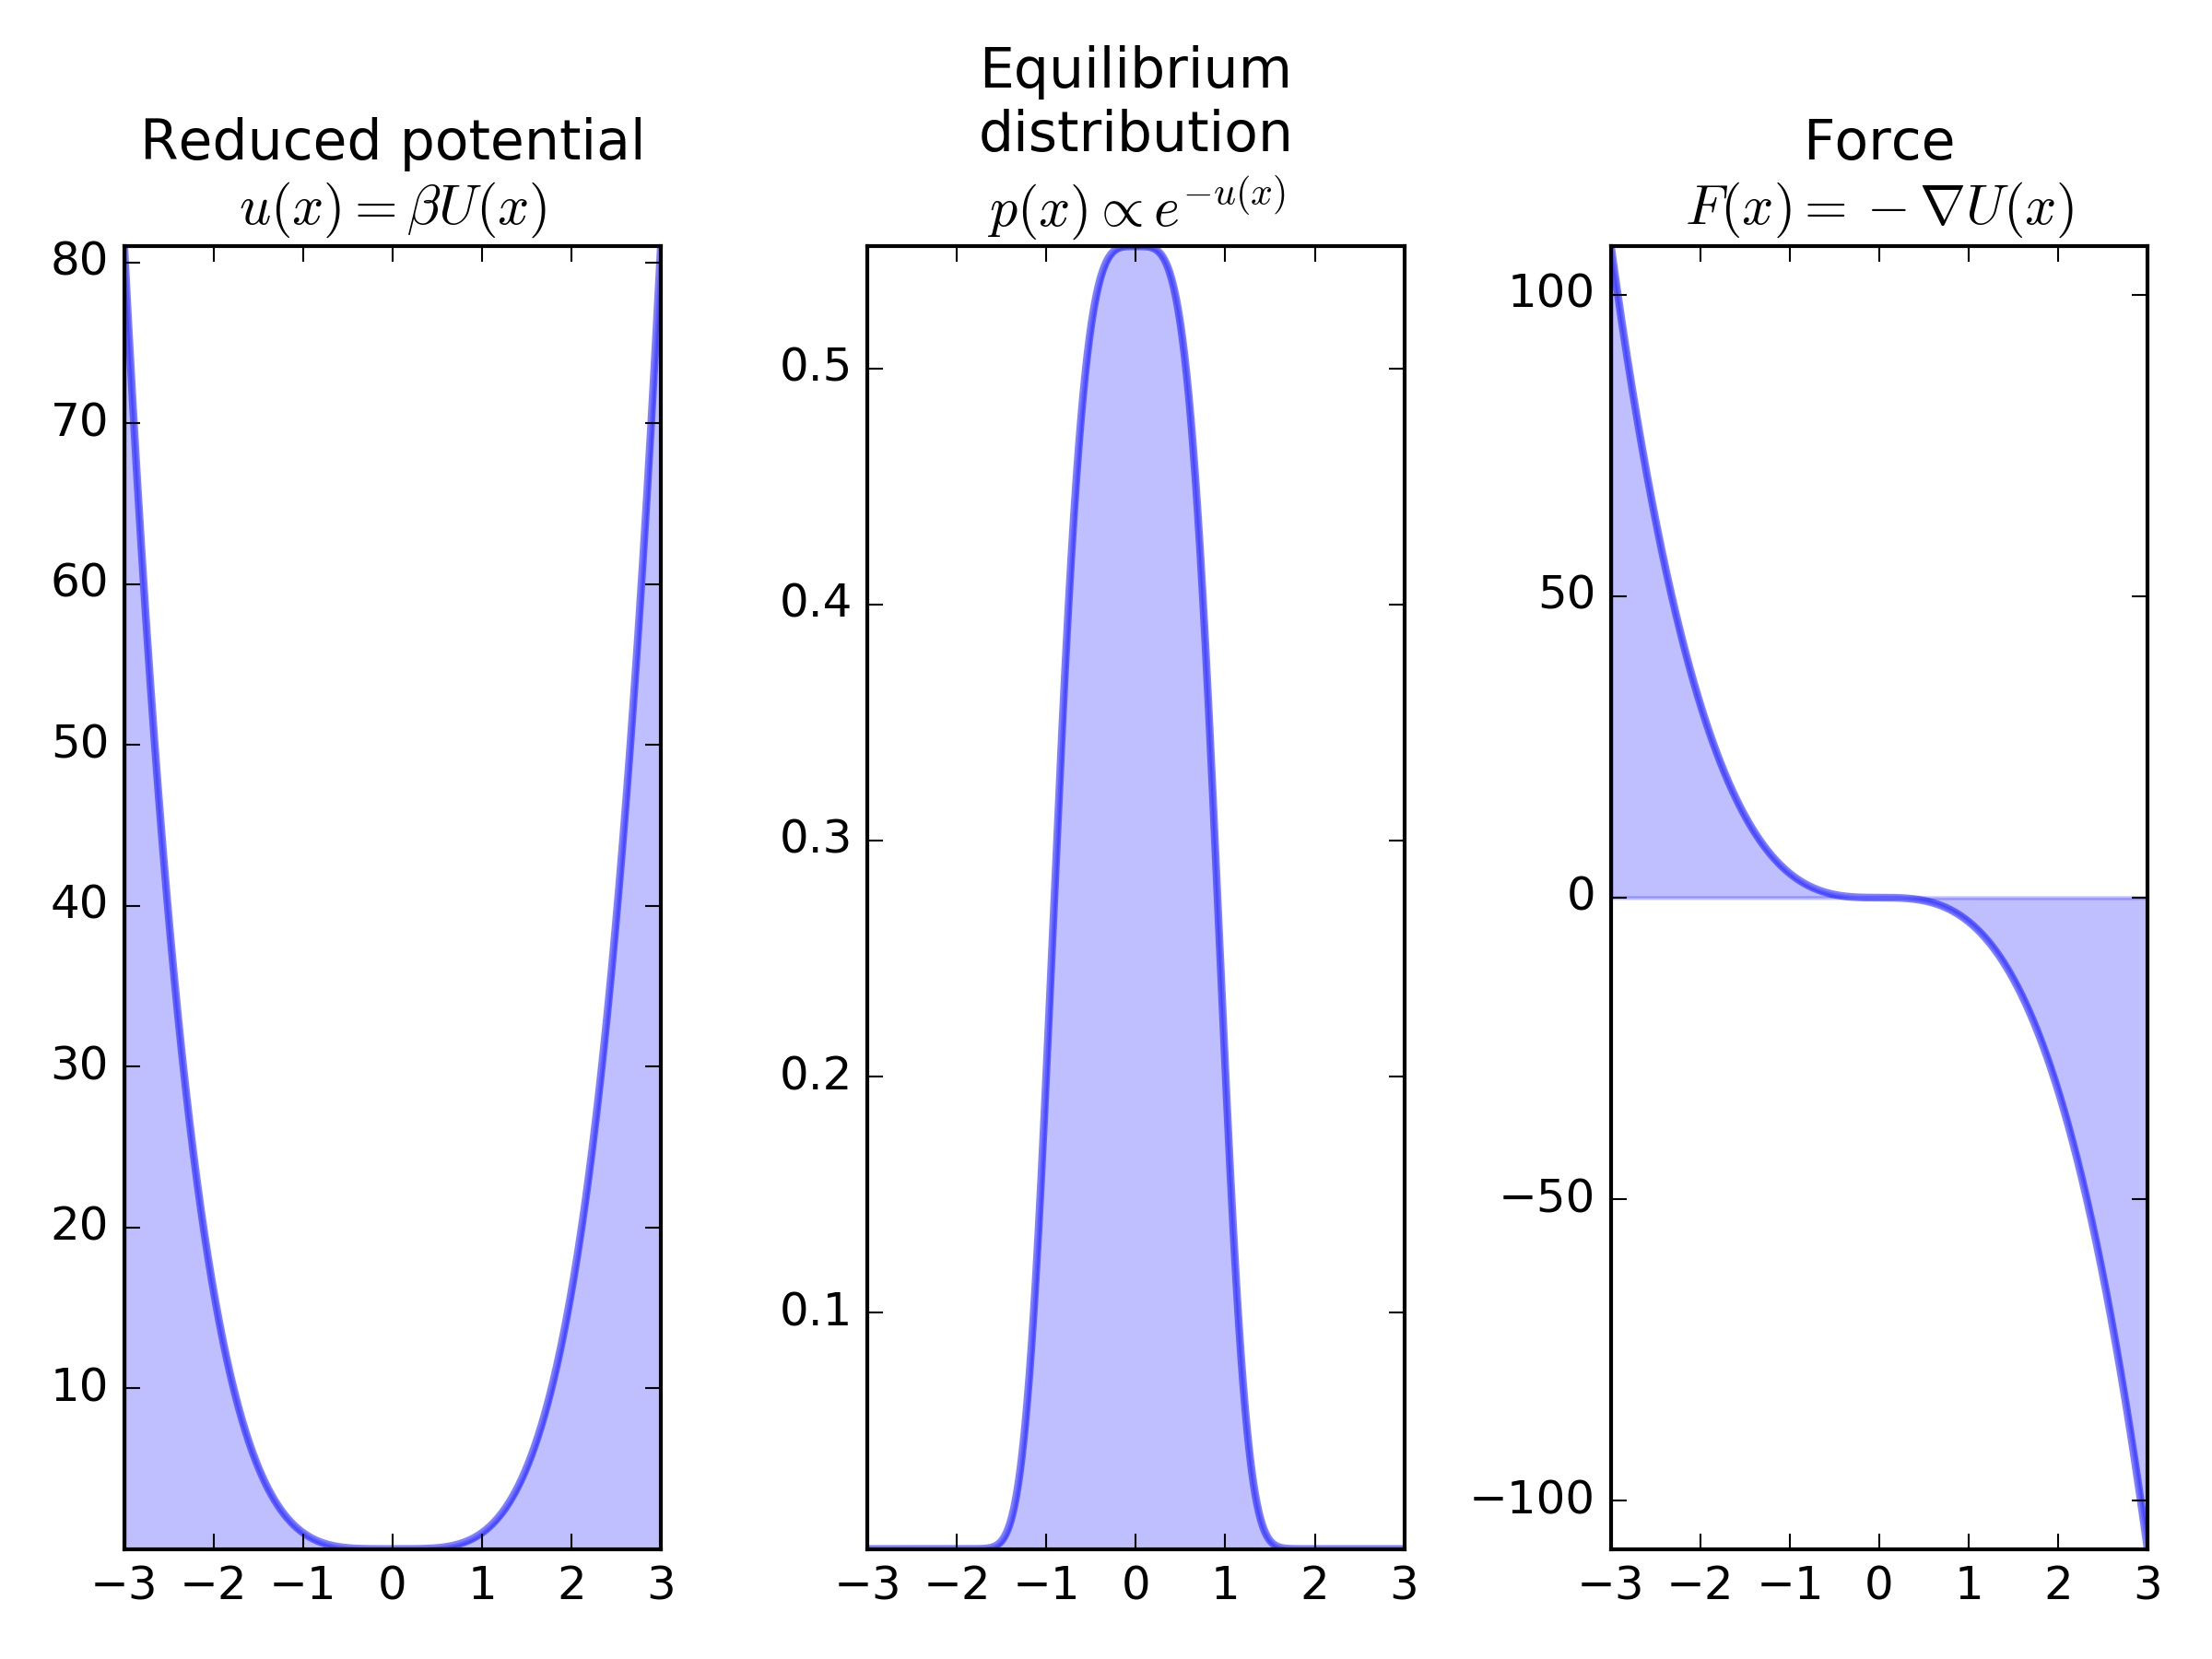
\includegraphics[width=0.5\textwidth]{quartic_system.jpg}
\end{figure}

\subsection{Methods}
Code to reproduce these experiments is available on Github: \url{https://github.com/choderalab/integrator-benchmark/tree/master/code/toy}.

\begin{enumerate}
\item \textbf{System definition:} Quartic potential $U(x) = x^4$, mass $m=10$, inverse temperature $\beta = 1$, friction $\gamma = 100$, tested timestep range $0.25-1.1$ (stability limit of VVVR for this system appears to be about $1.2$).
\item \textbf{Generating equilibrium and steady state samples} For each condition, I run the integrator for 100 million steps, and save every 100th $(x,v)$ snapshot. To generate equilibrium samples, I run 100 million steps of random-walk Metropolis-Hastings with standard Normal proposals.
\item \textbf{Estimating ``ground-truth'' KL divergence.} I used two methods to measure the KL divergence between the Langevin steady state and equilibrium:
\begin{enumerate}
\item \textit{Estimate as a free energy difference,} $\kldiv( \conf(x) \| p(x) ) = (\langle U(x) \rangle_\text{neq} - S_\text{neq} -  (\langle U(x) \rangle_\text{eq} - S_\text{eq})$. Where $\langle U(x) \rangle_\text{neq} \approx \frac{1}{N} \sum_{i=1}^N U(x^{(i)})$ is estimated as the sample mean of the potential energy over the steady-state samples $x^{(i)}$, $S_\text{neq}$ is the entropy of a 200-bin histogram of the steady-state $x$ samples, and $\langle U(x) \rangle_\text{eq}$ and $S_\text{eq}$ are computed using numerical quadrature.
\item \textit{Estimate as the KL divergence between histograms} of the sampled nonequilibrium steady state vs. the exact histogram of the equilibrium $x$ distribution over those same bins.
\end{enumerate}
These estimates agree to about 4 decimal places, so I just plot the second estimate in all subsequent figures.
Perhaps cleverer baseline estimators of the KL divergence would be helpful.
\item \textbf{Nonequilibrium protocol} Draw an equilibrium sample $(x,v) \sim \pi$, apply the Langevin integrator for $M=200$ steps to produce $(x', v') \sim \rho$. Record shadow work accumulated during that trajectory as $W_{\pi \to \rho}$. Randomize $v'' \sim q$, so that $(x', v'') \sim \omega$. Apply the integrator for $M$ steps, record shadow work performed by the second trajectory as $W_{\omega \to \rho}$. Perform 1 million such protocols, and report $\hat{\kldiv}(\conf \| p) \approx \frac{\beta}{2} [ \langle W_{\pi \to \rho} \rangle - \langle W_{\omega \to \rho} \rangle ]$.
\end{enumerate}

\subsection{Results}

\subsubsection{Validating $\kldiv$ estimator}
First, we compare the proposed nonequilibrium estimator of the KL divergence to the precise numerical computation of the KL divergence.

% estimator comparison
\begin{figure}[h]
	\centering
	% note: fix this file name
	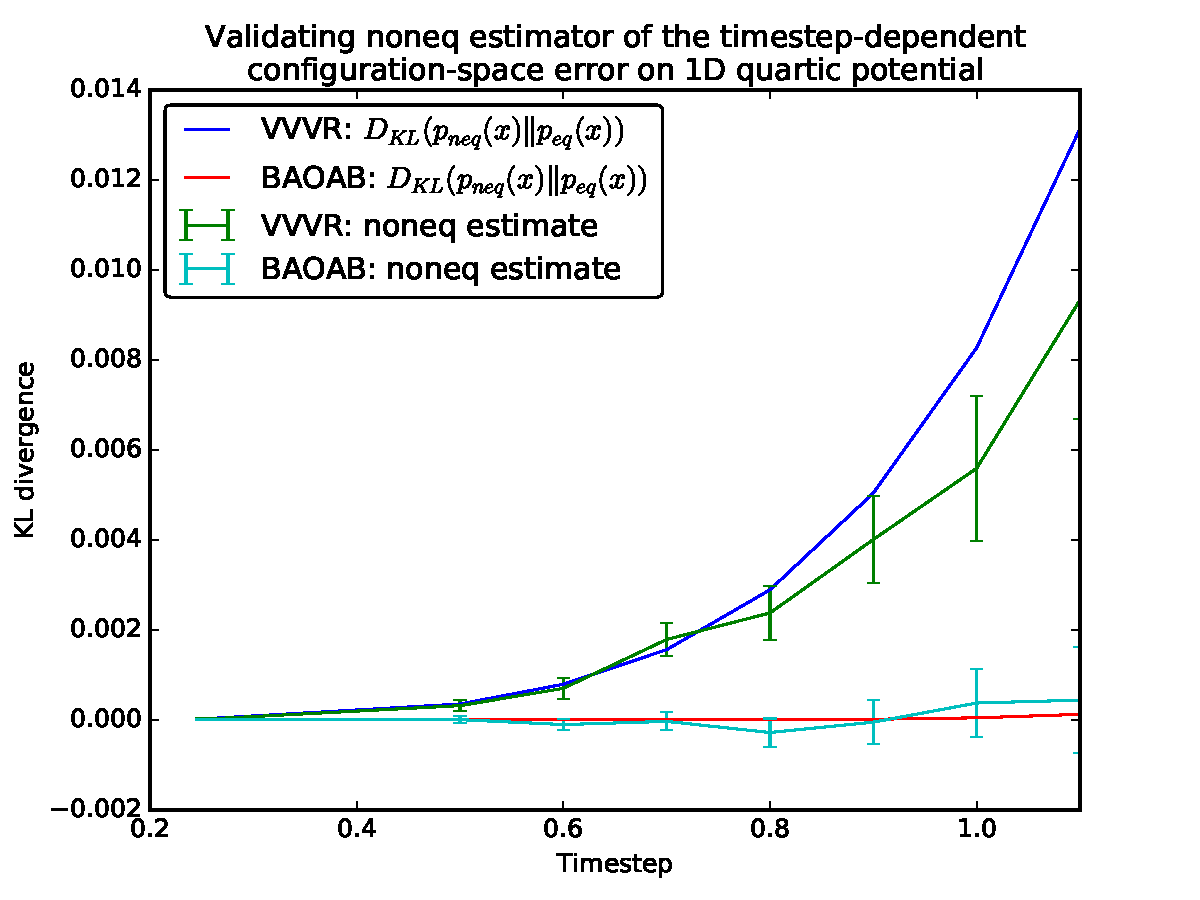
\includegraphics[width=0.5\textwidth]{estimator_comparison.pdf}
	\caption{Estimator comparison}
\end{figure}

The estimator was within error of the correct answer for 14 of 16 points on this plot.
The variance of the naive estimator, even with a million protocol samples, is very high.

\subsubsection{Examining the sampled distributions}
For this system, BAOAB has extremely low configuration-space bias even up to the stability limit (but doesn't preserve the velocity distribution as well), while VVVR has extremely low velocity bias (but doesn't preserve the configuration distribution as well).
At the maximum timestep tested, the configuration-space bias of VVVR was about 100 times greater than that of BAOAB ($\kldiv(\conf^\text{BAOAB} \| p) \approx 0.00013$, and $\kldiv(\conf^\text{VVVR} \| p) \approx 0.01309$).

% x samples
\begin{figure}[H] % x samples VVVR
    \centering
    \begin{subfigure}[b]{0.3\textwidth}
        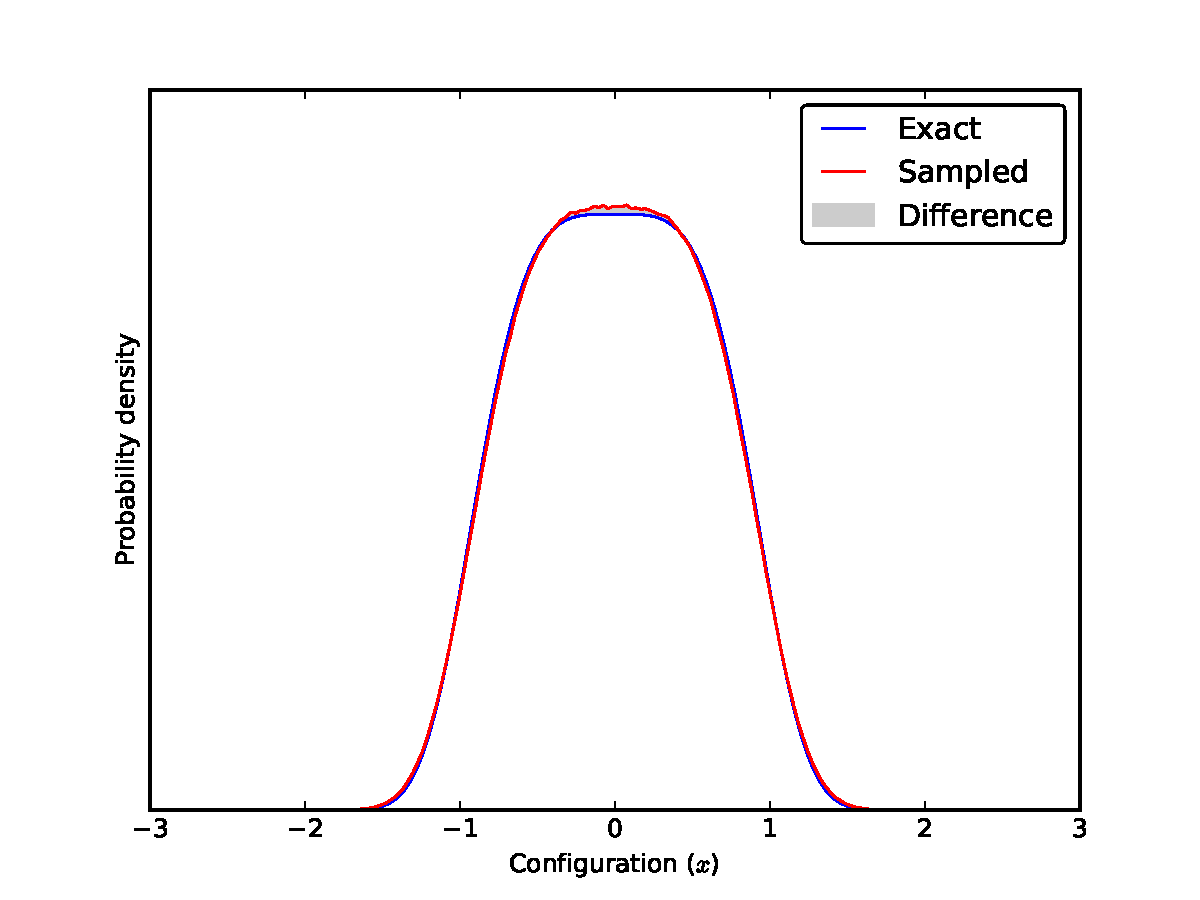
\includegraphics[width=\textwidth]{x_samples_VVVR_dt=0-5.pdf}
        \caption{$\delta t = 0.5$}
    \end{subfigure}
    \begin{subfigure}[b]{0.3\textwidth}
        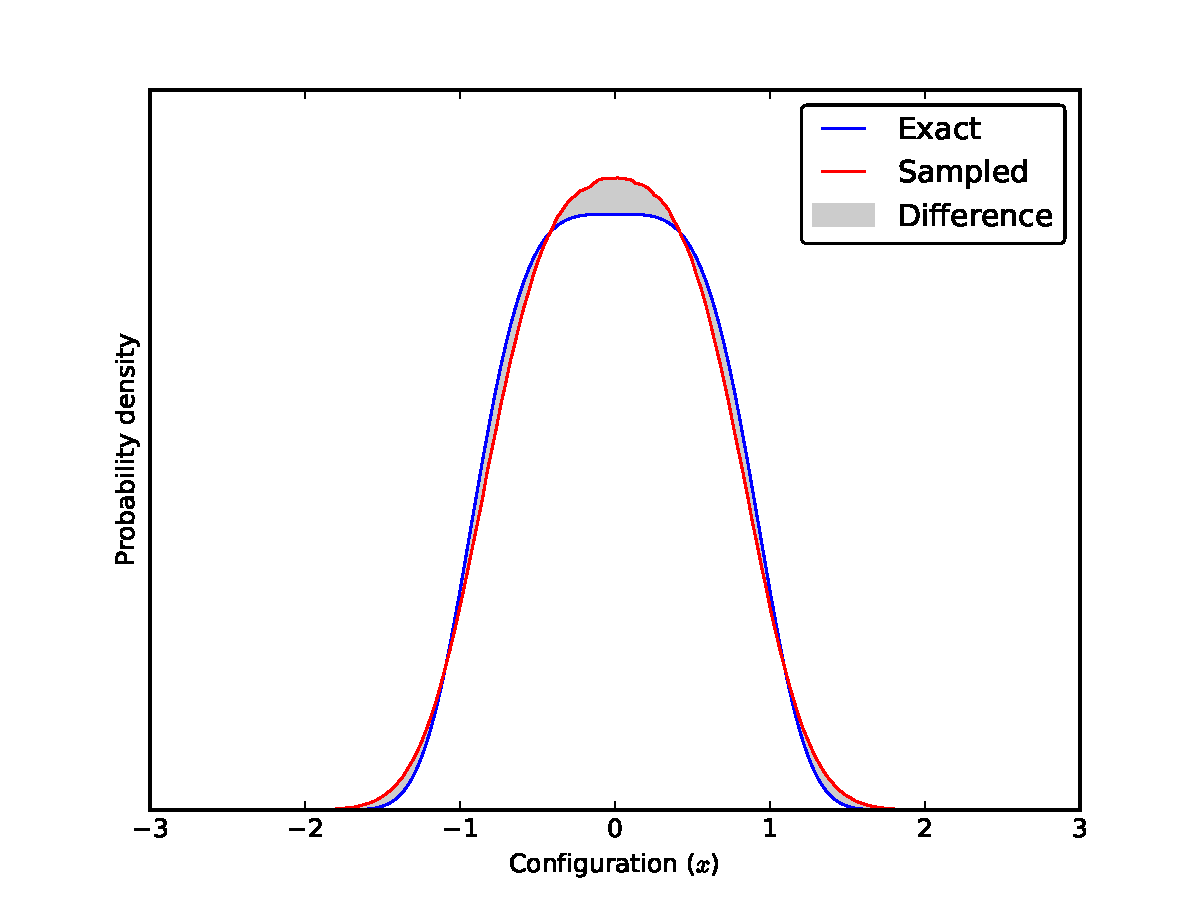
\includegraphics[width=\textwidth]{x_samples_VVVR_dt=1-0.pdf}
        \caption{$\delta t = 1$}
    \end{subfigure}
    \begin{subfigure}[b]{0.3\textwidth}
        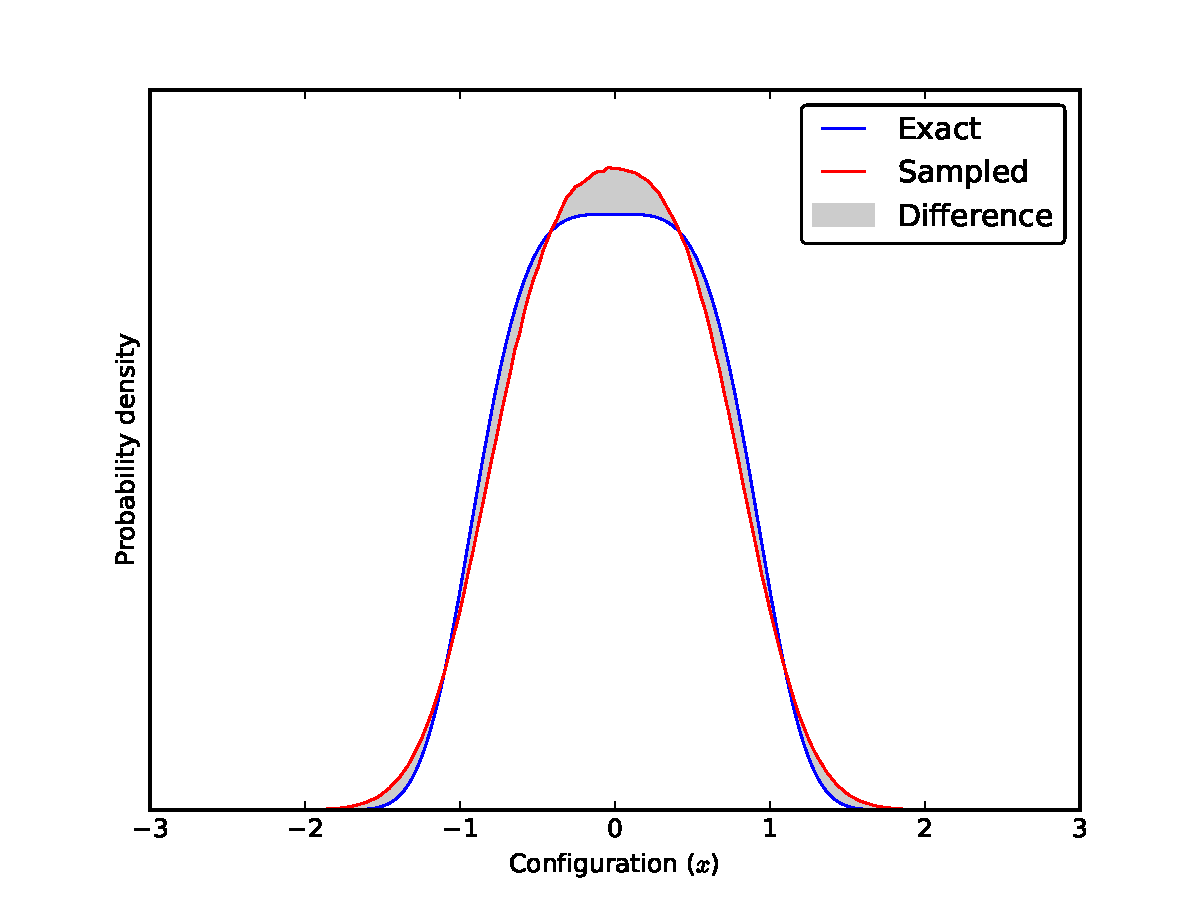
\includegraphics[width=\textwidth]{x_samples_VVVR_dt=1-1.pdf}
        \caption{$\delta t = 1.1$}
    \end{subfigure}
    \caption{VVVR sampled configuration distribution}
\end{figure}

\begin{figure}[H] % x samples BAOAB
    \centering
    \begin{subfigure}[b]{0.3\textwidth}
        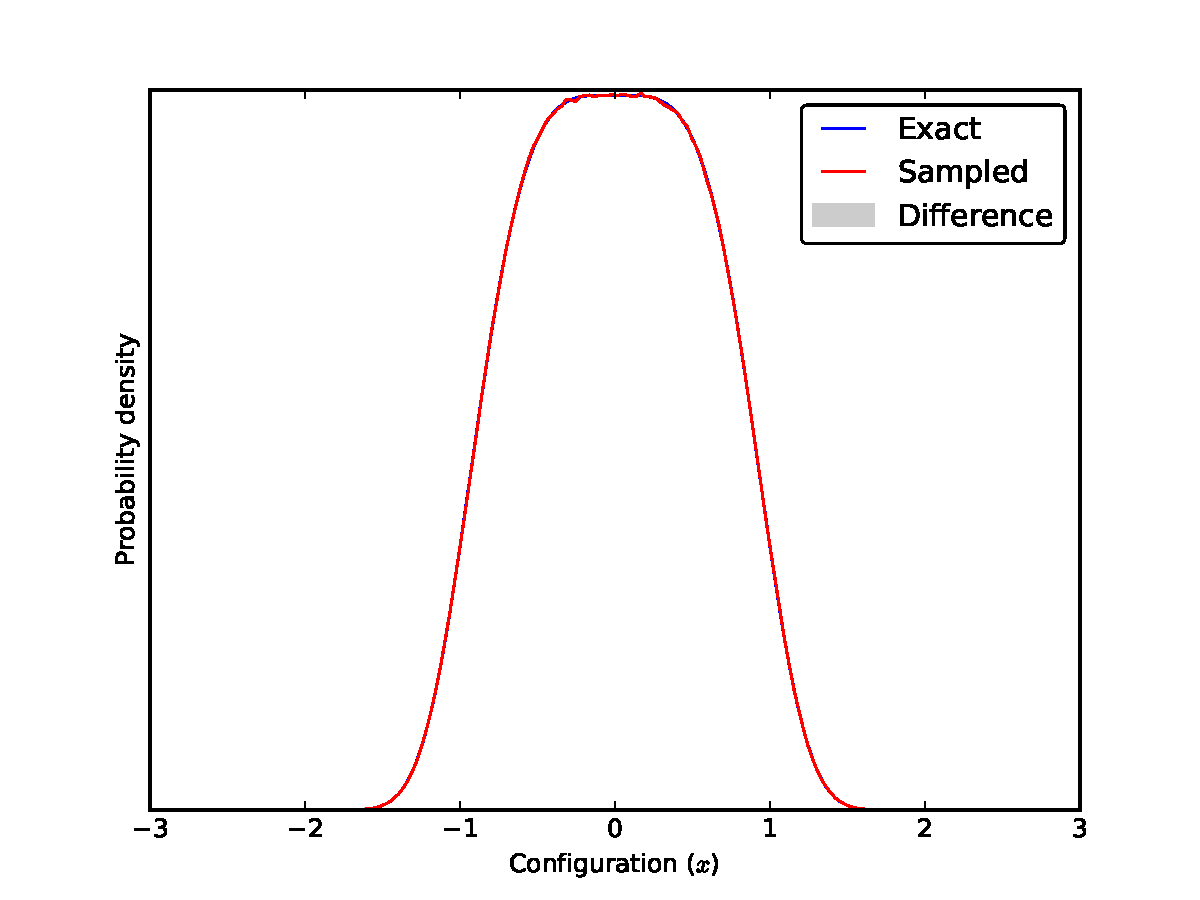
\includegraphics[width=\textwidth]{x_samples_BAOAB_dt=0-5.pdf}
        \caption{$\delta t = 0.5$}
    \end{subfigure}
    \begin{subfigure}[b]{0.3\textwidth}
        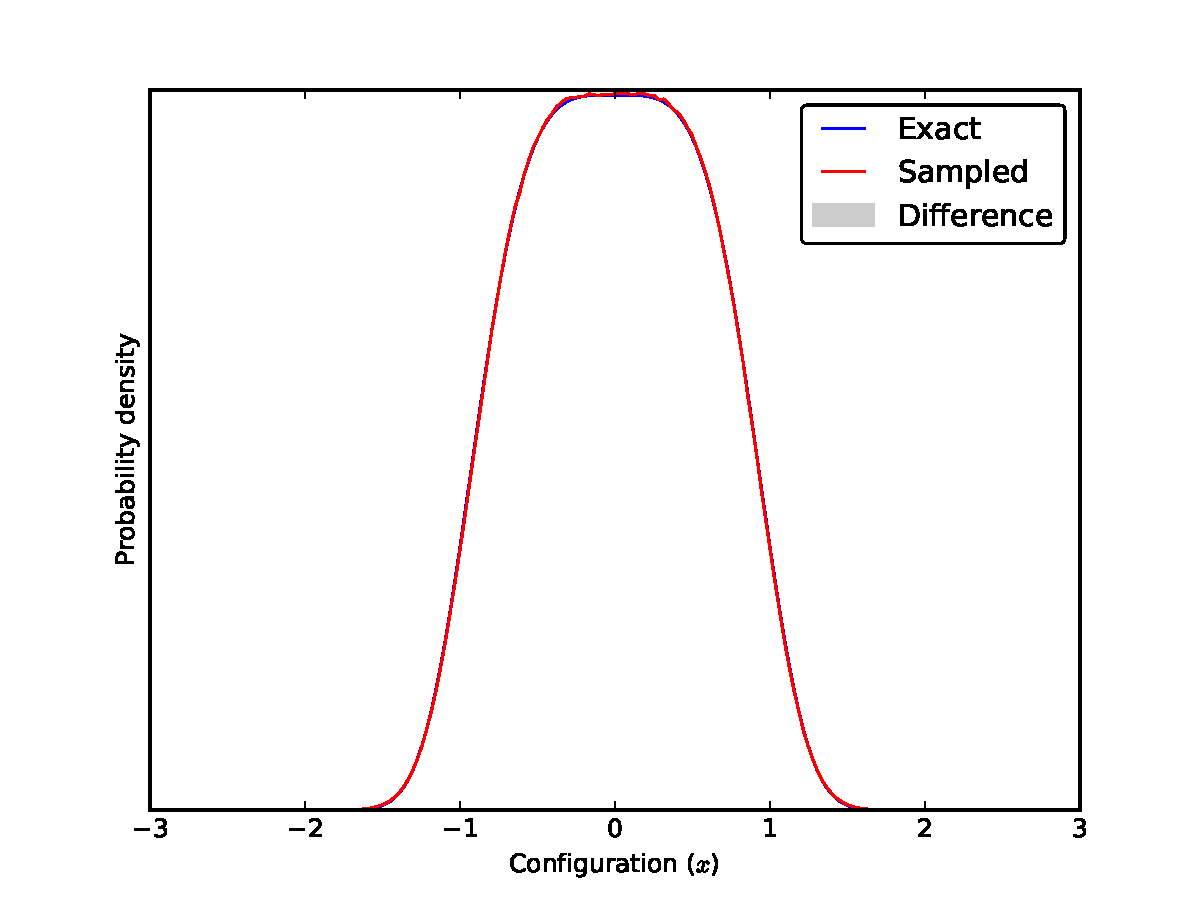
\includegraphics[width=\textwidth]{x_samples_BAOAB_dt=1-0.pdf}
        \caption{$\delta t = 1$}
    \end{subfigure}
    \begin{subfigure}[b]{0.3\textwidth}
        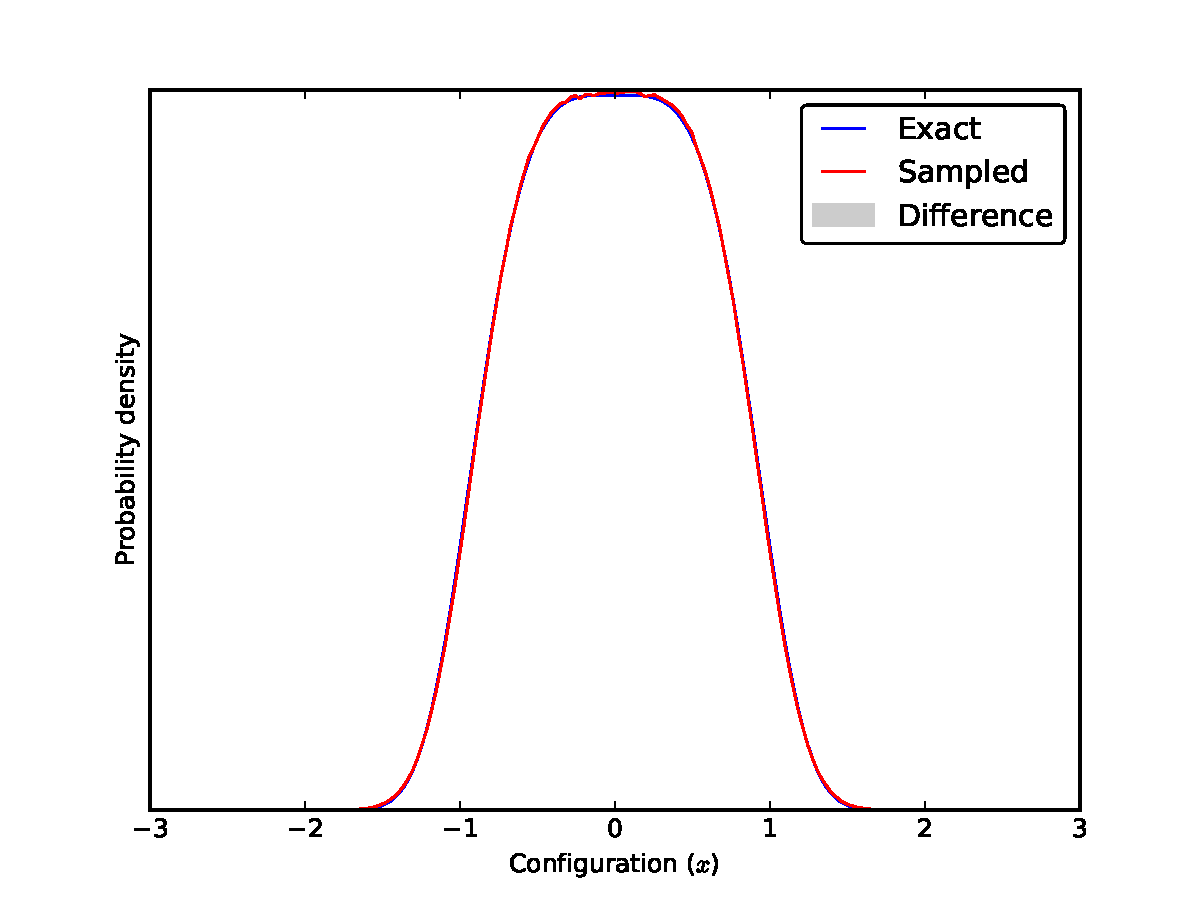
\includegraphics[width=\textwidth]{x_samples_BAOAB_dt=1-1.pdf}
        \caption{$\delta t = 1.1$}
    \end{subfigure}
    \caption{BAOAB sampled configuration distribution}
\end{figure}

% v samples
\begin{figure}[H] % v samples VVVR
    \centering
    \begin{subfigure}[b]{0.3\textwidth}
        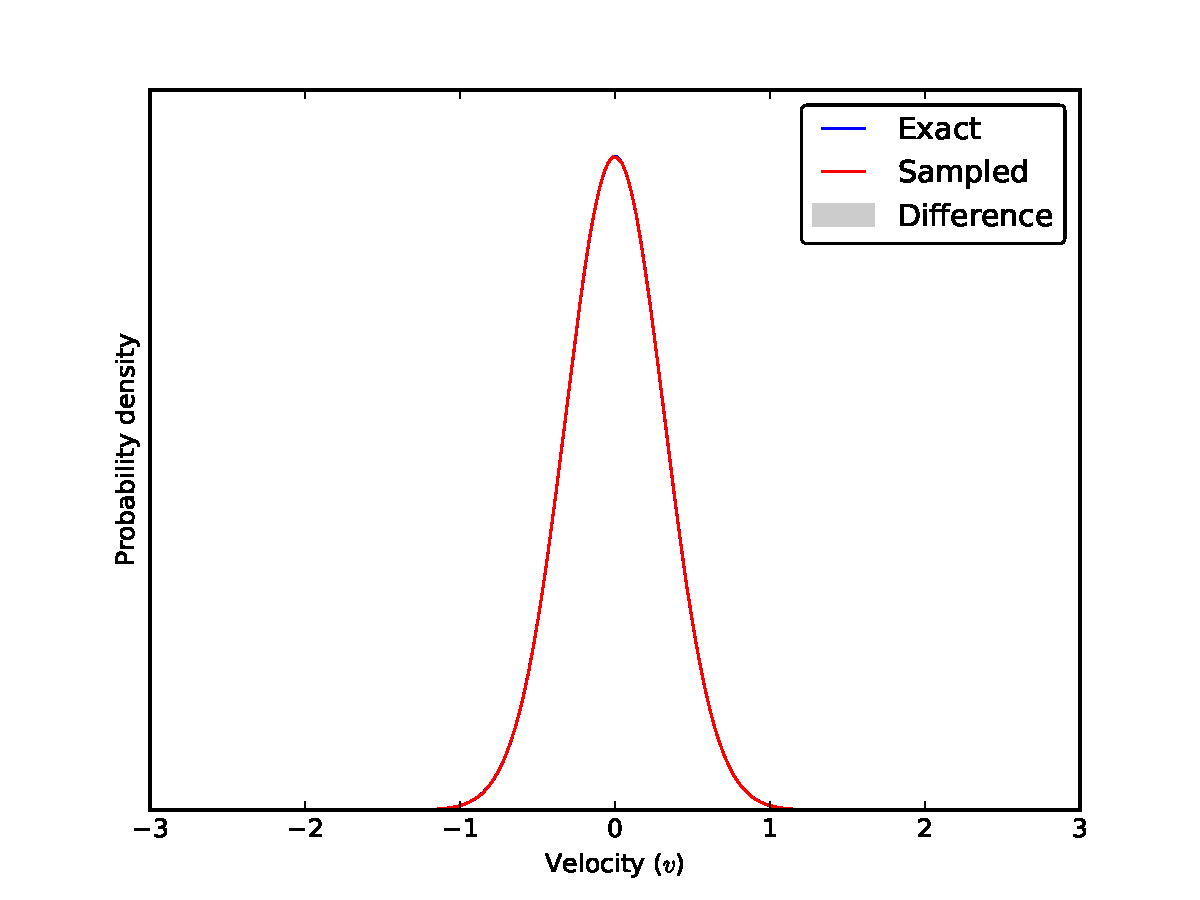
\includegraphics[width=\textwidth]{v_samples_VVVR_dt=0-5.pdf}
        \caption{$\delta t = 0.5$}
    \end{subfigure}
    \begin{subfigure}[b]{0.3\textwidth}
        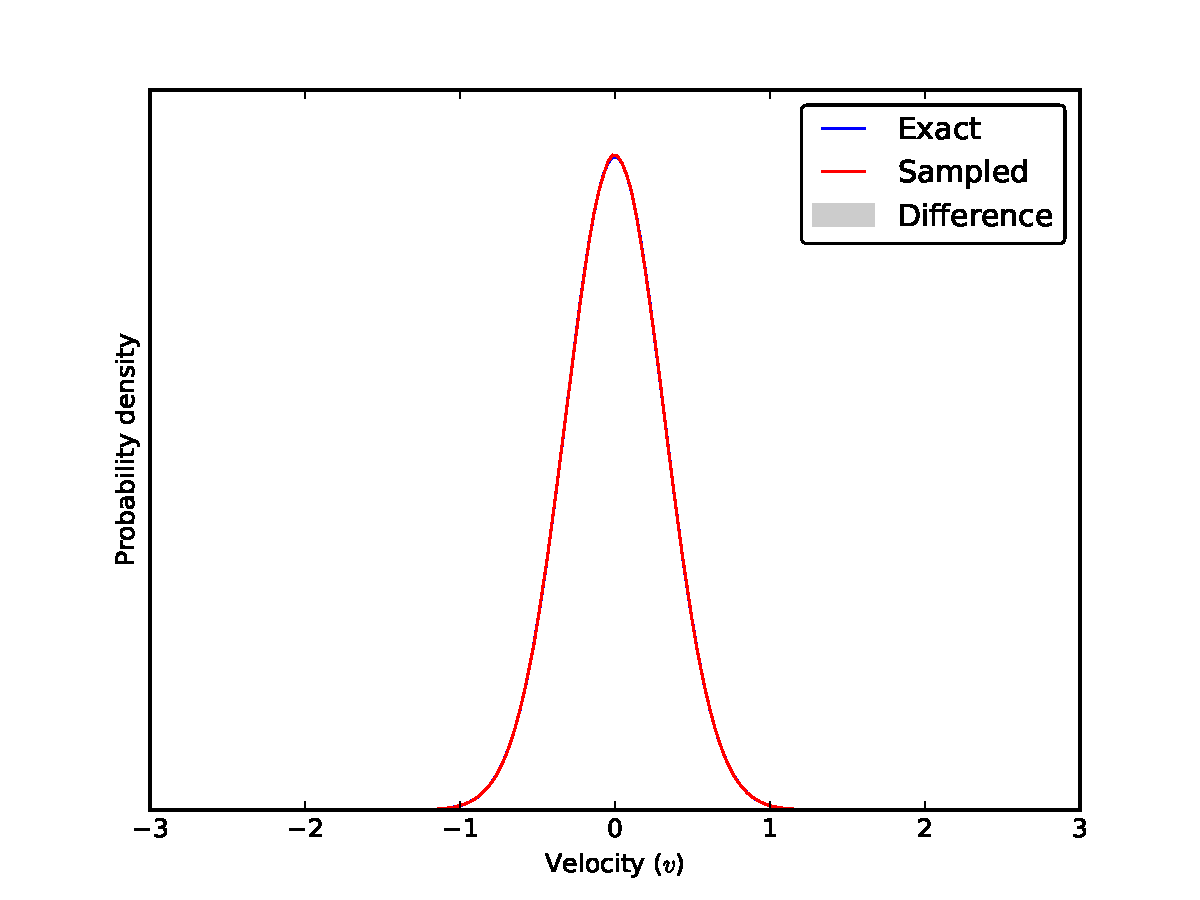
\includegraphics[width=\textwidth]{v_samples_VVVR_dt=1-0.pdf}
        \caption{$\delta t = 1$}
    \end{subfigure}
    \begin{subfigure}[b]{0.3\textwidth}
        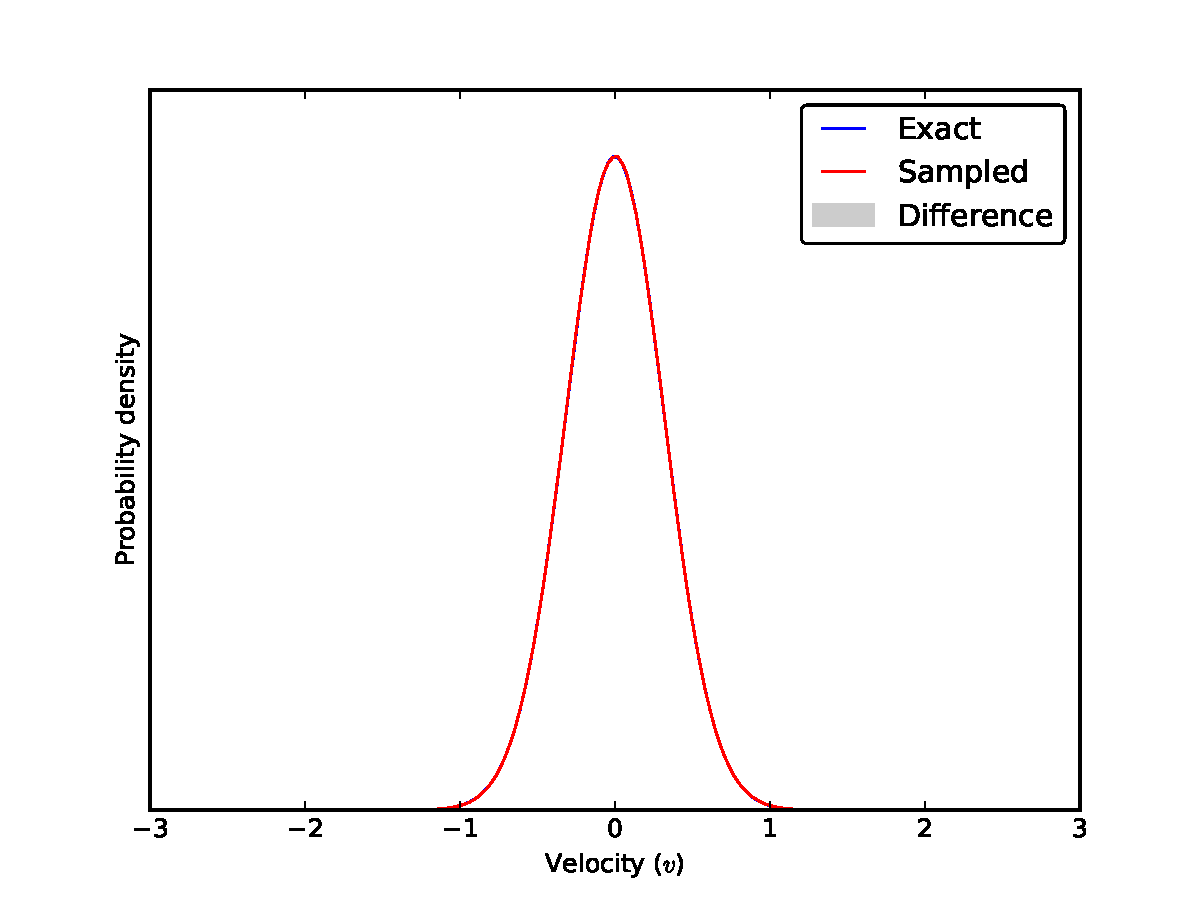
\includegraphics[width=\textwidth]{v_samples_VVVR_dt=1-1.pdf}
        \caption{$\delta t = 1.1$}
    \end{subfigure}
    \caption{VVVR sampled velocity distribution}
\end{figure}
\begin{figure}[H] % v samples BAOAB
    \centering
    \begin{subfigure}[b]{0.3\textwidth}
        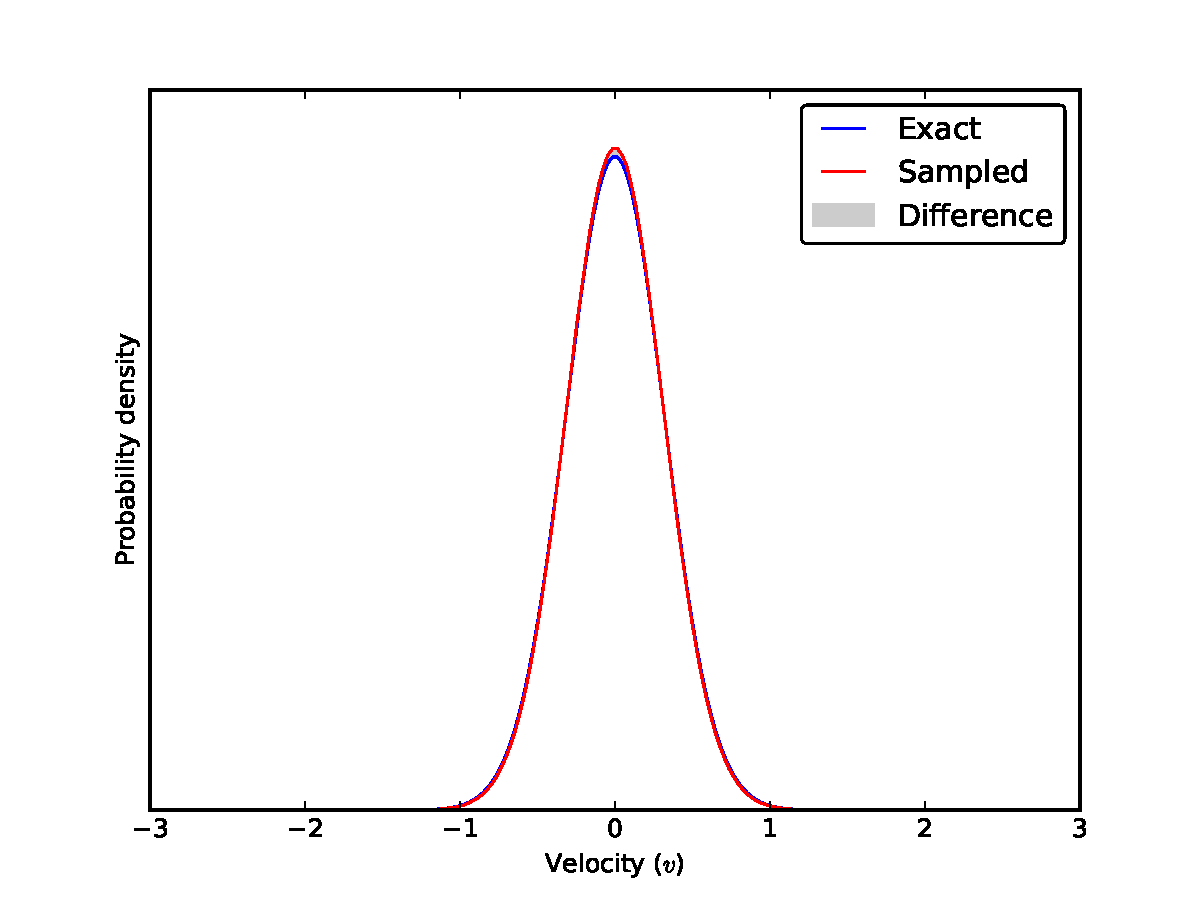
\includegraphics[width=\textwidth]{v_samples_BAOAB_dt=0-5.pdf}
        \caption{$\delta t = 0.5$}
    \end{subfigure}
    \begin{subfigure}[b]{0.3\textwidth}
        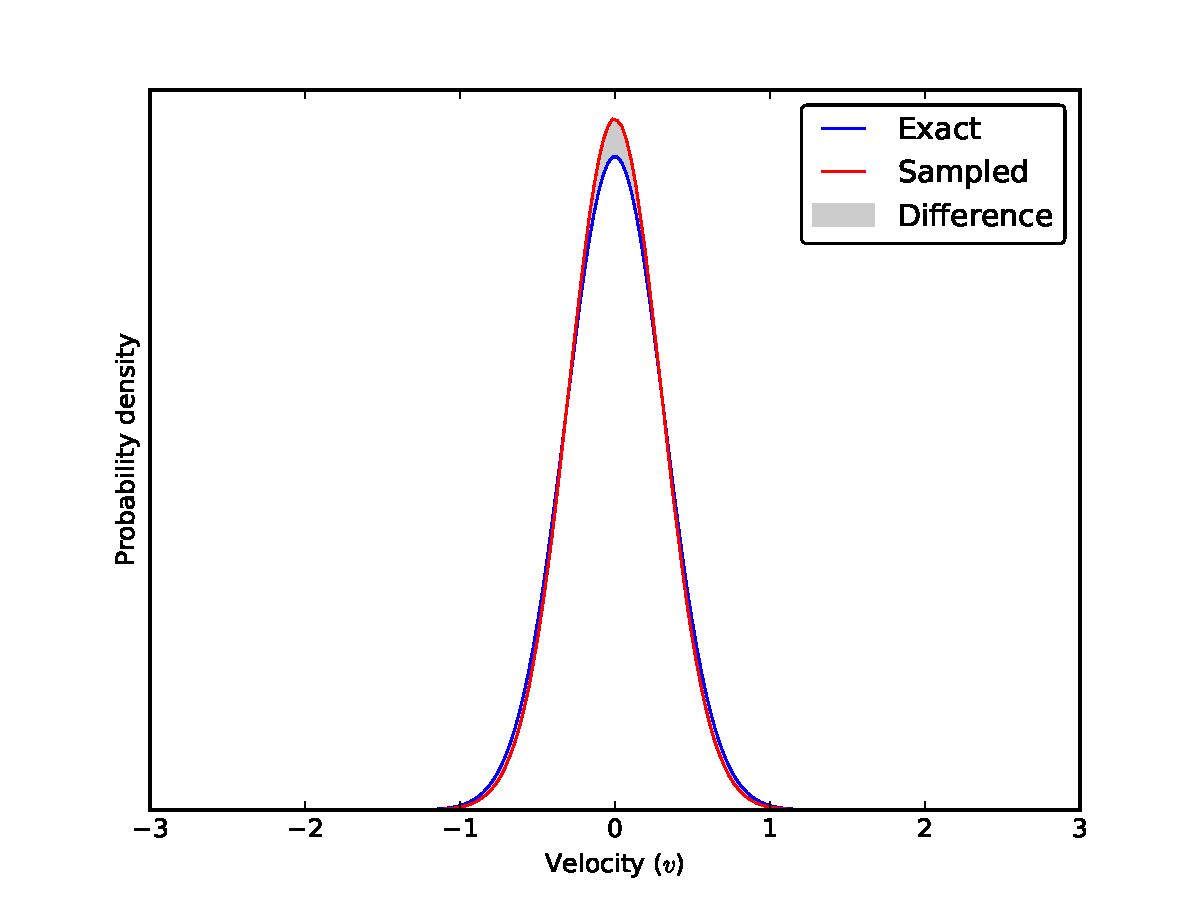
\includegraphics[width=\textwidth]{v_samples_BAOAB_dt=1-0.pdf}
        \caption{$\delta t = 1$}
    \end{subfigure}
    \begin{subfigure}[b]{0.3\textwidth}
        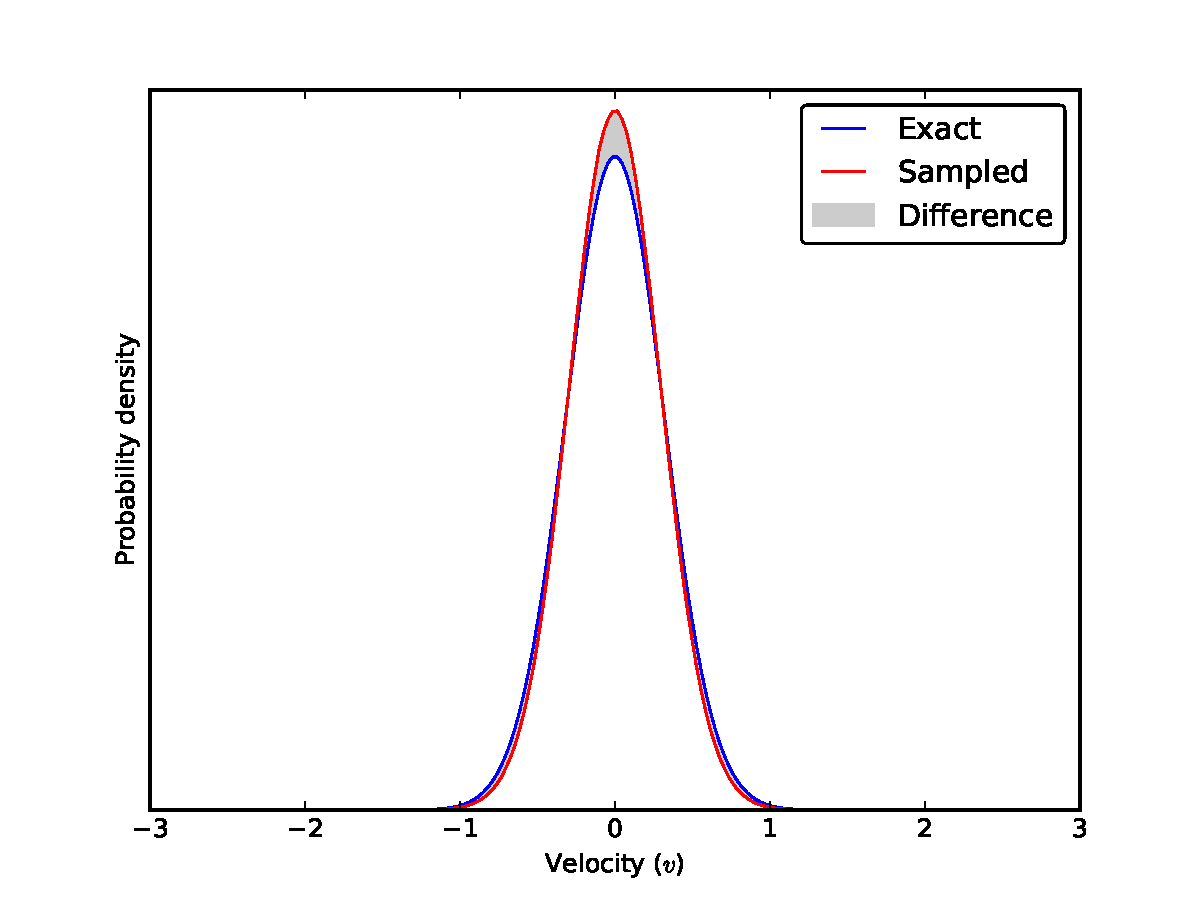
\includegraphics[width=\textwidth]{v_samples_BAOAB_dt=1-1.pdf}
        \caption{$\delta t = 1.1$}
    \end{subfigure}
    \caption{BAOAB sampled velocity distribution}
\end{figure}

Distortions in the velocity distribution sampled by BAOAB and the configuration distribution sampled by VVVR are visible in the plots above.


\subsubsection{Examining work trajectories}
% work trajectories
To visually confirm that we've reached the nonequilibrium steady state within $M=200$ integrator steps, we can inspect plots of the accumulated shadow work over time (note that the y-axes have different scales at each of the 3 timesteps.
\begin{figure}[h] % baoab work trajectories
    \centering
    \begin{subfigure}[b]{0.3\textwidth}
        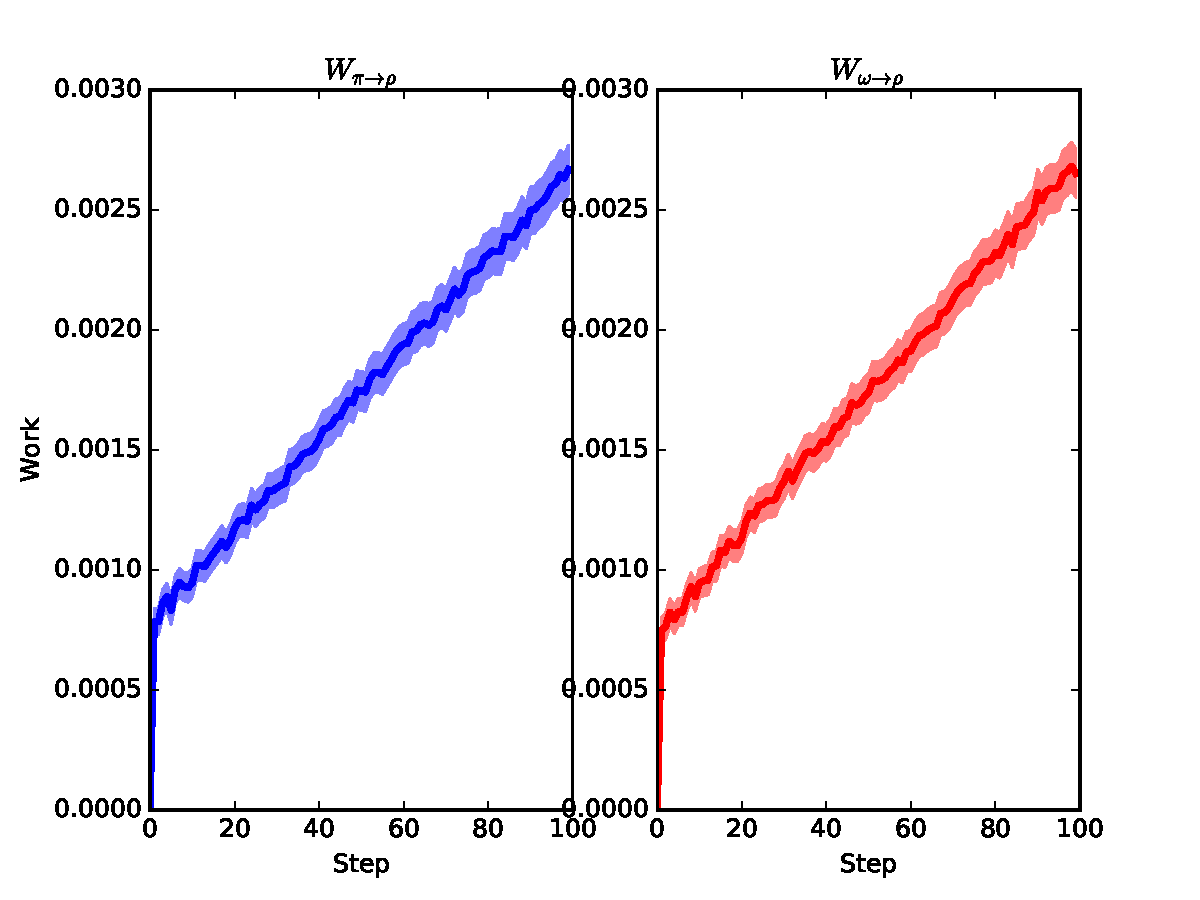
\includegraphics[width=\textwidth]{work_trajs_BAOAB_dt=0-5.pdf}
        \caption{$\delta t = 0.5$}
    \end{subfigure}
    \begin{subfigure}[b]{0.3\textwidth}
        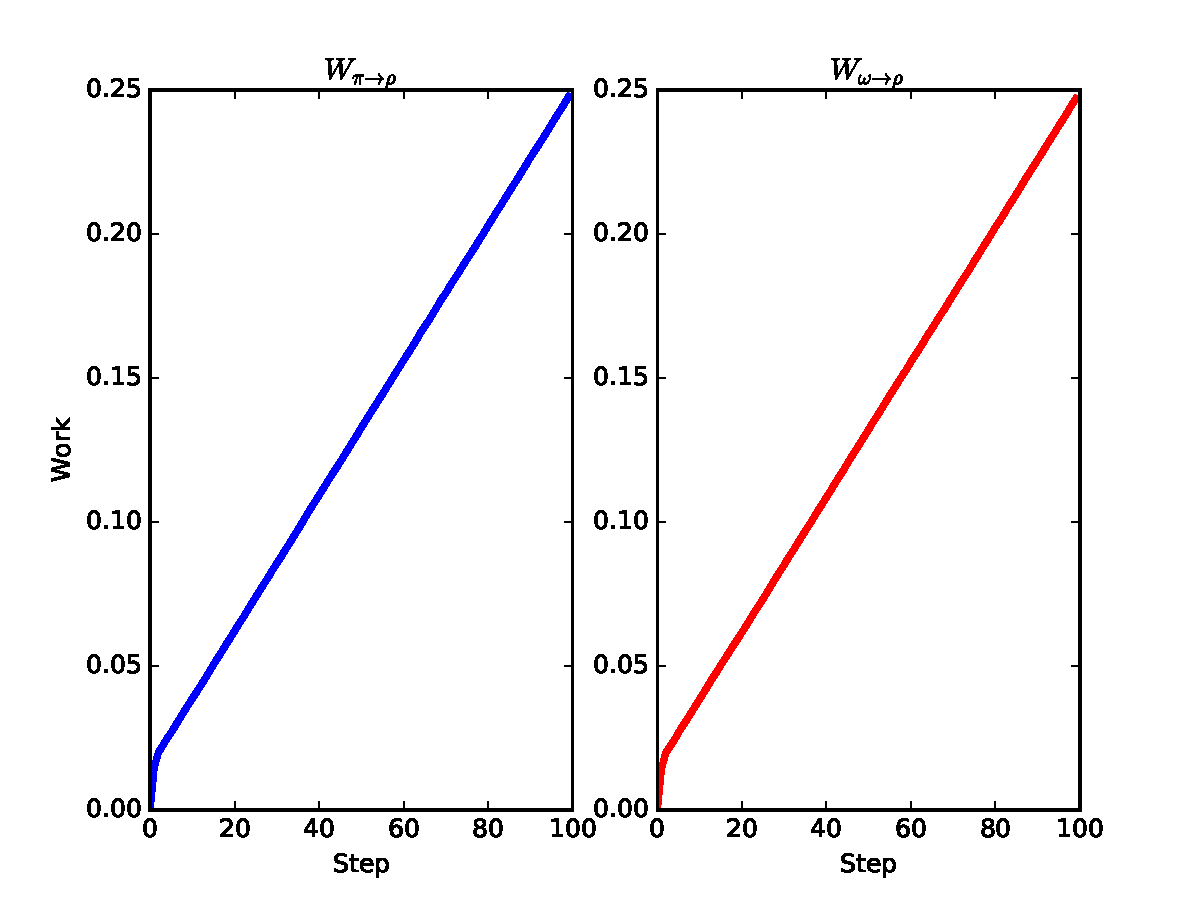
\includegraphics[width=\textwidth]{work_trajs_BAOAB_dt=1-0.pdf}
        \caption{$\delta t = 1$}
    \end{subfigure}
    \begin{subfigure}[b]{0.3\textwidth}
        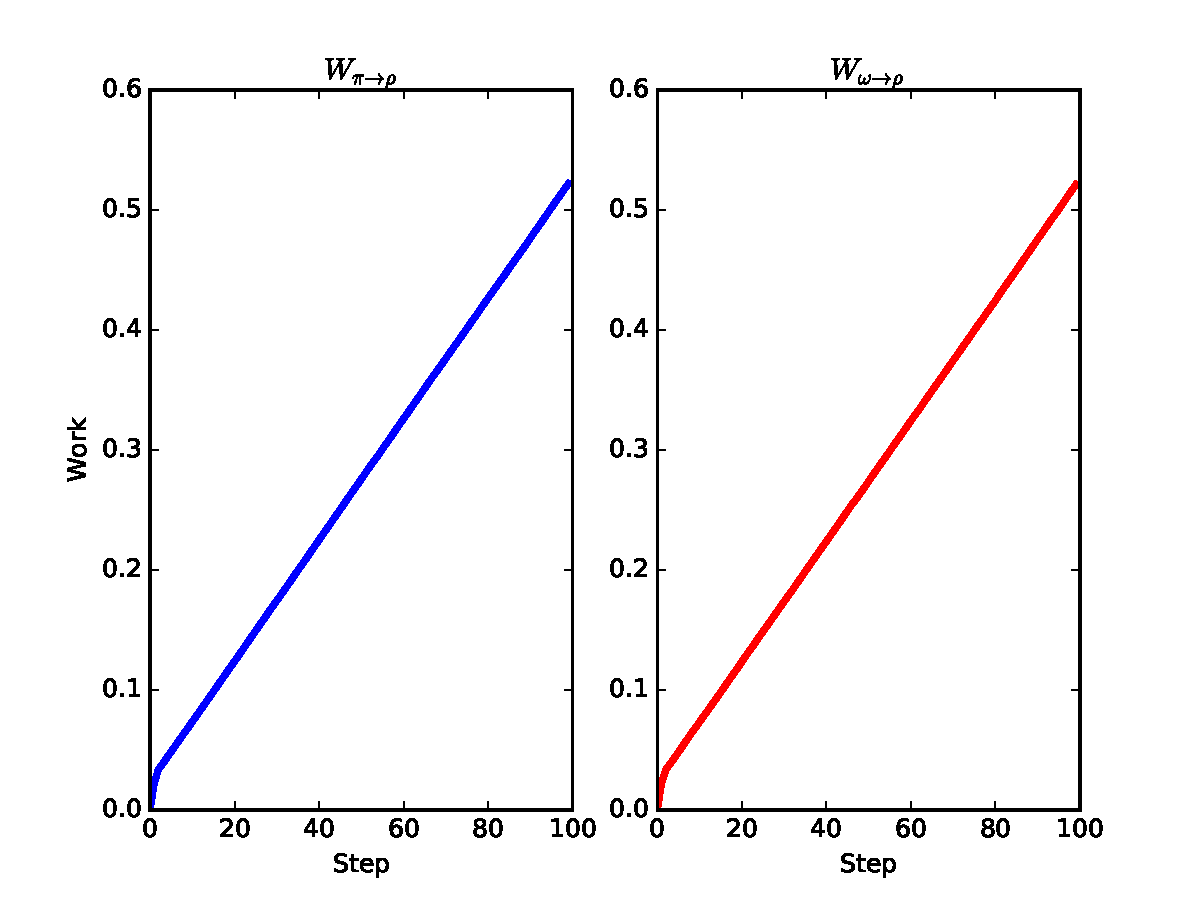
\includegraphics[width=\textwidth]{work_trajs_BAOAB_dt=1-1.pdf}
        \caption{$\delta t = 1.1$}
    \end{subfigure}
    \caption{BAOAB work trajectories}
\end{figure}

\begin{figure}[h] % vvvr work trajectories
    \centering
    \begin{subfigure}[b]{0.3\textwidth}
        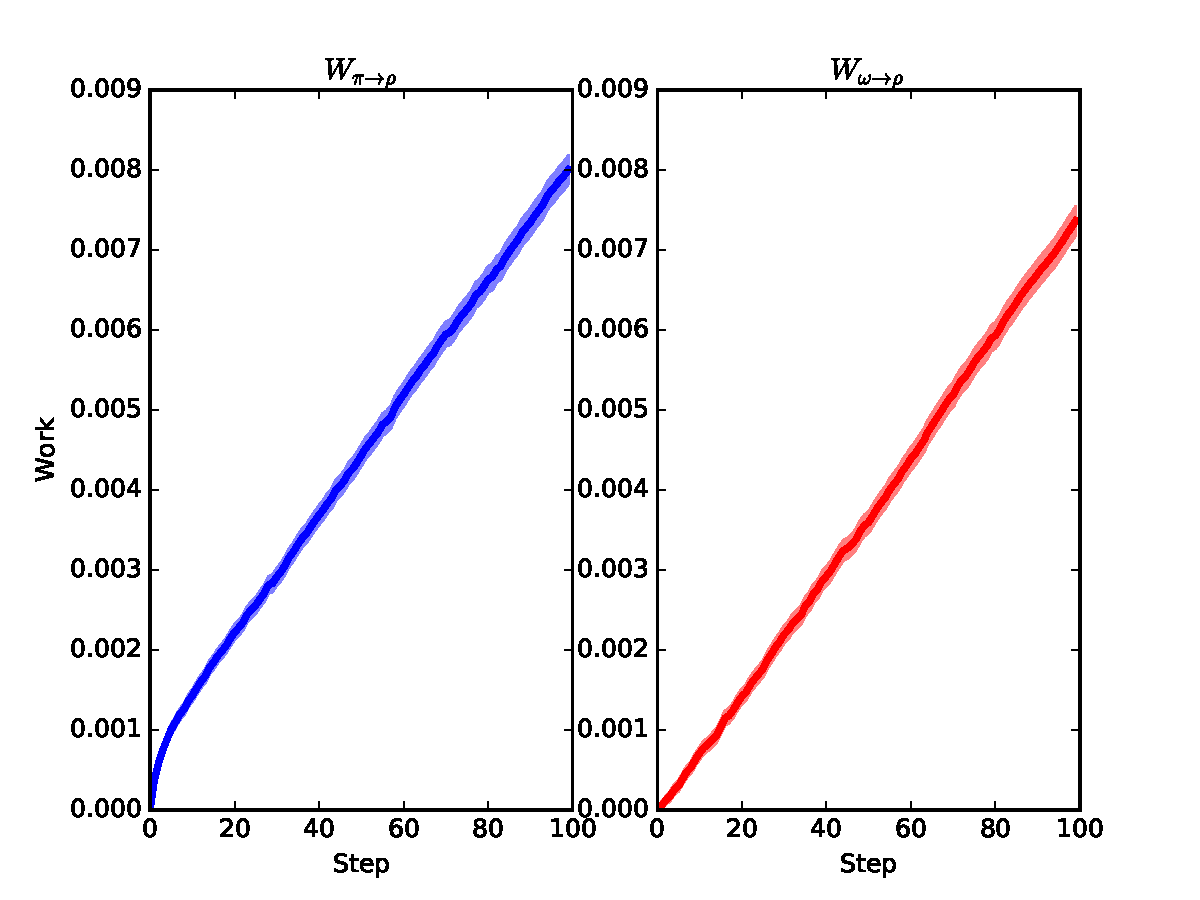
\includegraphics[width=\textwidth]{work_trajs_VVVR_dt=0-5.pdf}
        \caption{$\delta t = 0.5$}
    \end{subfigure}
    \begin{subfigure}[b]{0.3\textwidth}
        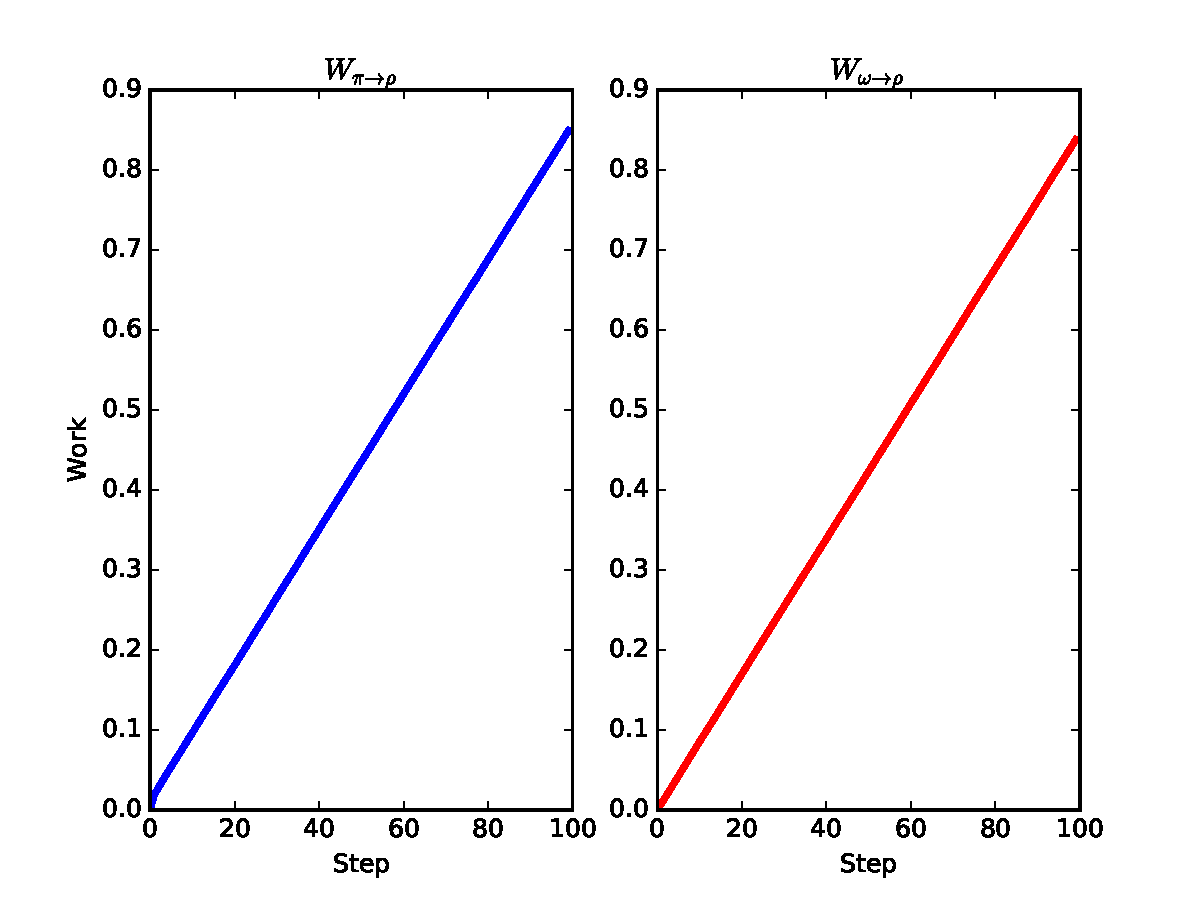
\includegraphics[width=\textwidth]{work_trajs_VVVR_dt=1-0.pdf}
        \caption{$\delta t = 1$}
    \end{subfigure}
    \begin{subfigure}[b]{0.3\textwidth}
        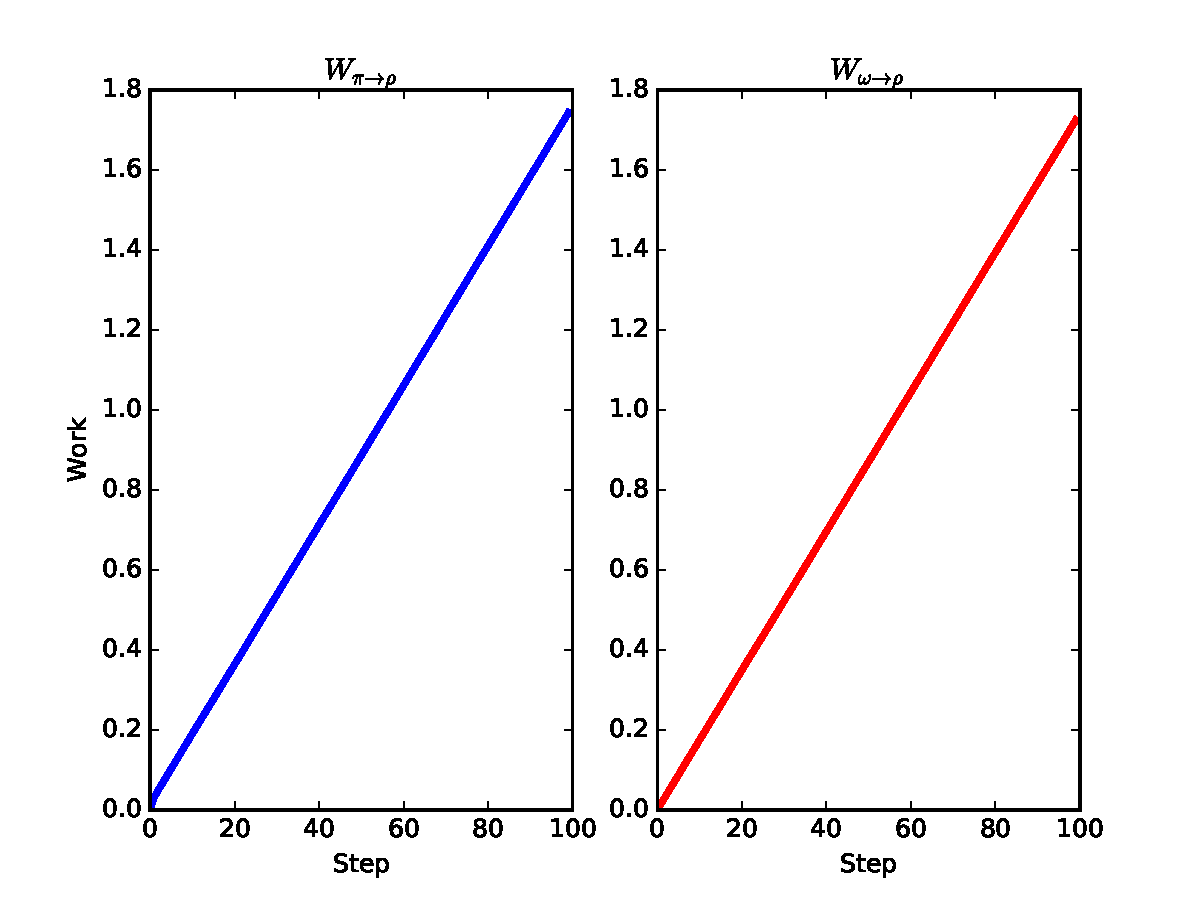
\includegraphics[width=\textwidth]{work_trajs_VVVR_dt=1-1.pdf}
        \caption{$\delta t = 1.1$}
    \end{subfigure}
    \caption{VVVR work trajectories}
\end{figure}

For this system, it looks like the nonequilibrium steady state is reached quite rapidly, and we could perhaps use the ``redundant'' information from, say, steps 10 through 200 of each trajectory to reduce the variance of our estimator.
I haven't yet explored this, but currently we use just a single number from each trajectory (the shadow work at the endpoint of the trajectory).

\subsubsection{Examining work distributions}
Next, we can inspect the distributions of shadow work at the end-points of each trajectory (note that the y-axis is log-scale).
% work distributions
\begin{figure}[h] % baoab work distributions
    \centering
    \begin{subfigure}[b]{0.3\textwidth}
        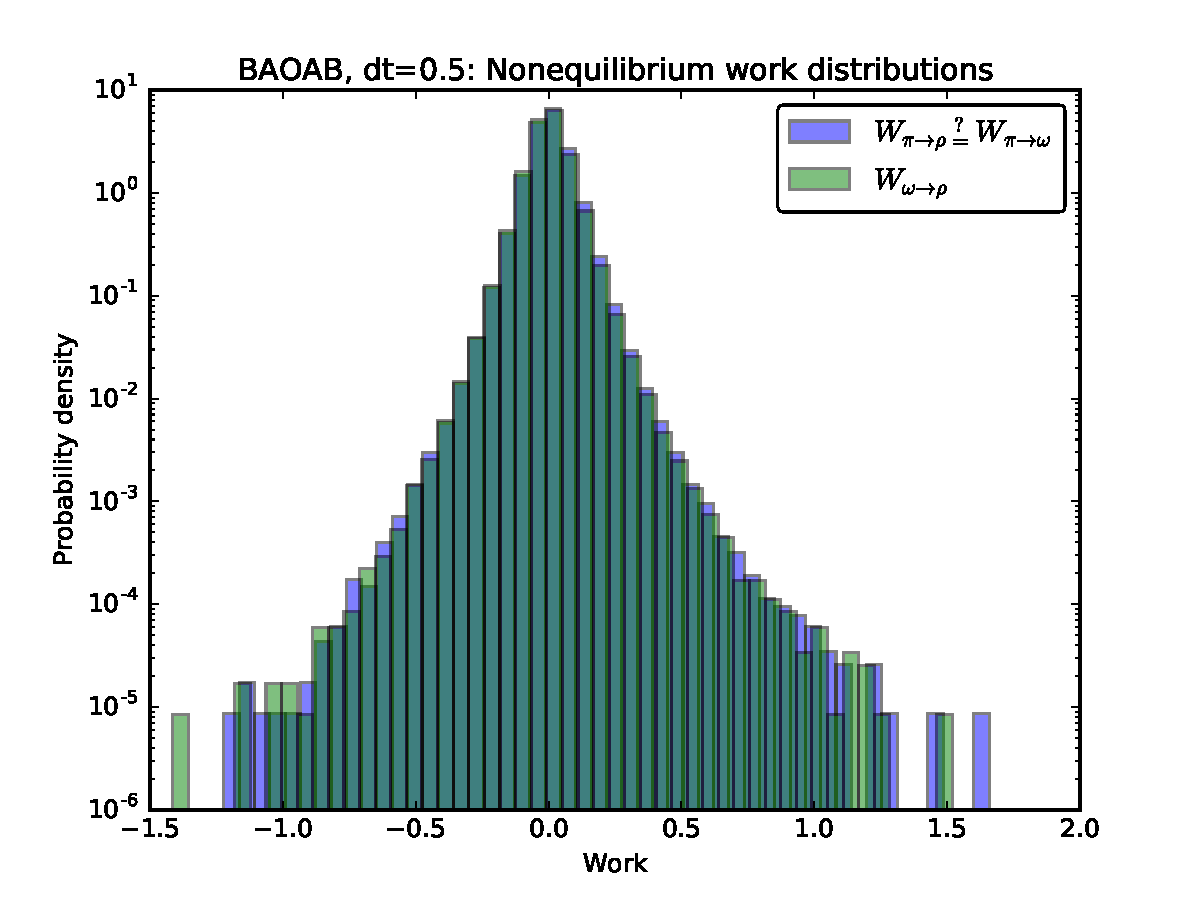
\includegraphics[width=\textwidth]{work_dists_BAOAB_dt=0-5.pdf}
        \caption{$\delta t = 0.5$}
    \end{subfigure}
    \begin{subfigure}[b]{0.3\textwidth}
        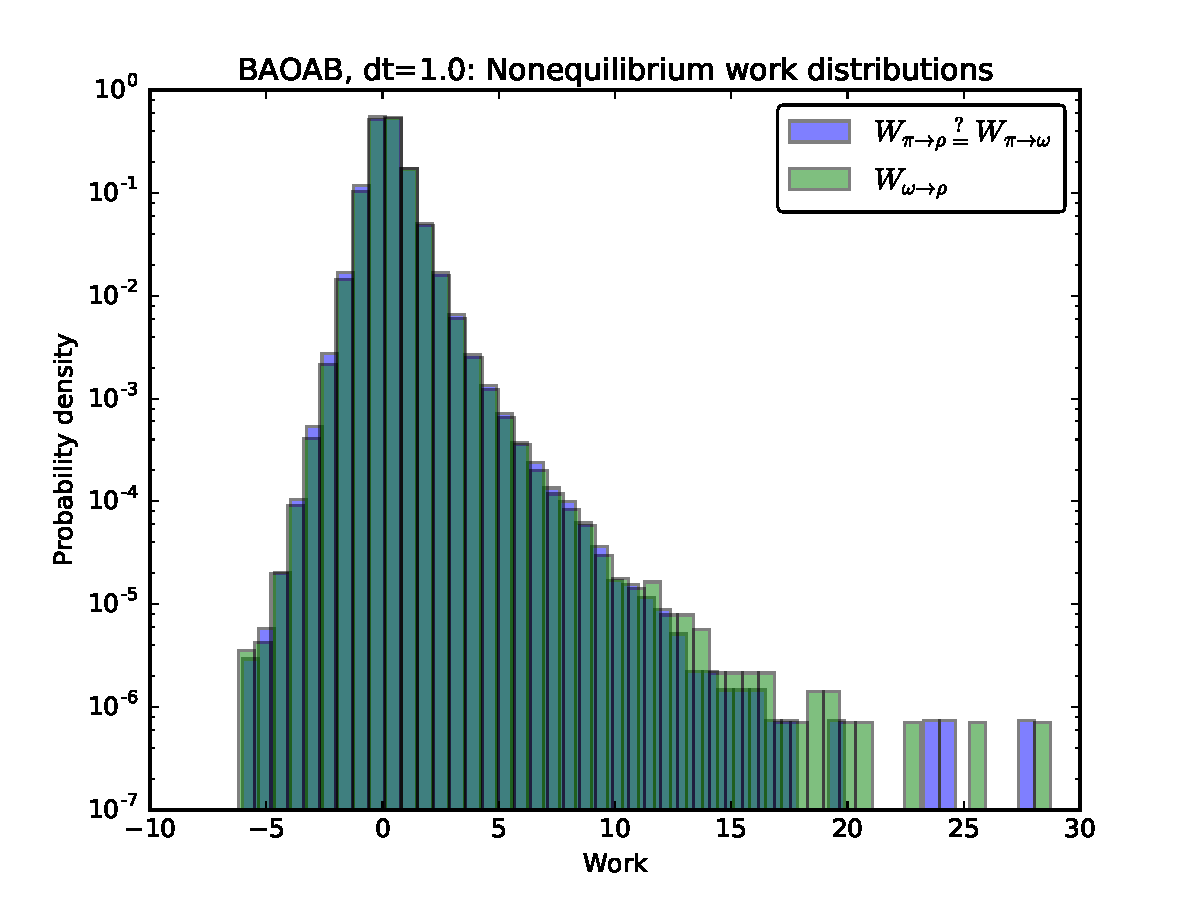
\includegraphics[width=\textwidth]{work_dists_BAOAB_dt=1-0.pdf}
        \caption{$\delta t = 1$}
    \end{subfigure}
    \begin{subfigure}[b]{0.3\textwidth}
        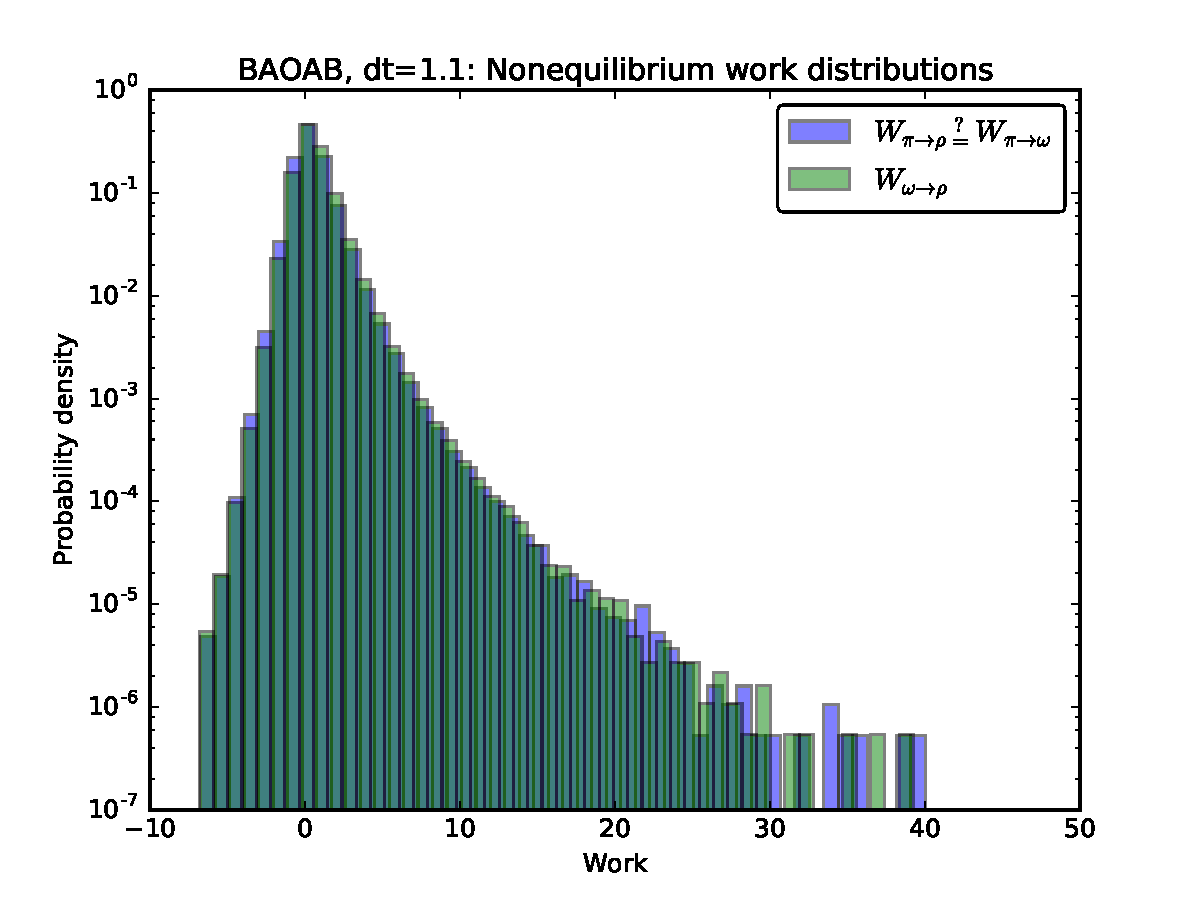
\includegraphics[width=\textwidth]{work_dists_BAOAB_dt=1-1.pdf}
        \caption{$\delta t = 1.1$}
    \end{subfigure}
    \caption{BAOAB work distributions}
\end{figure}
\begin{figure}[h] % vvvr work distributions
    \centering
    \begin{subfigure}[b]{0.3\textwidth}
        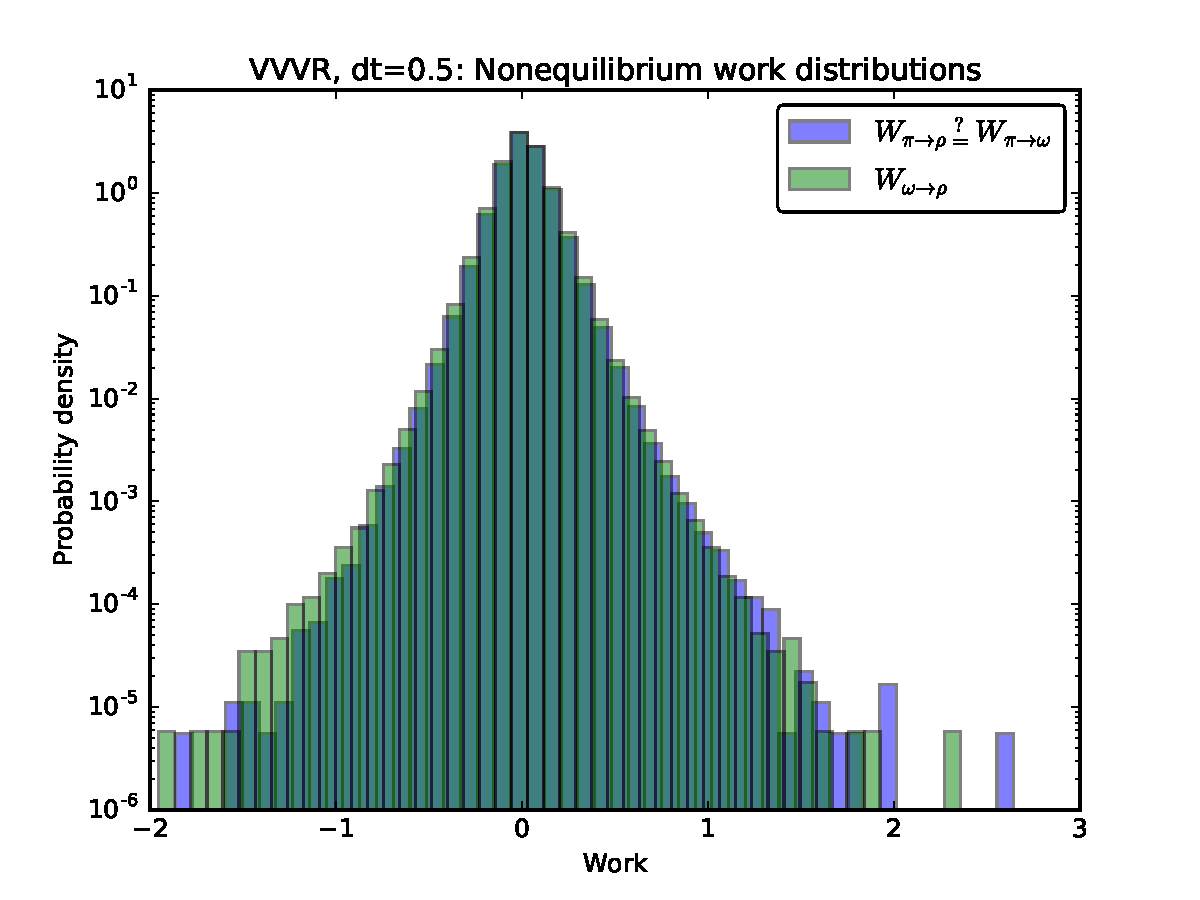
\includegraphics[width=\textwidth]{work_dists_VVVR_dt=0-5.pdf}
        \caption{$\delta t = 0.5$}
    \end{subfigure}
    \begin{subfigure}[b]{0.3\textwidth}
        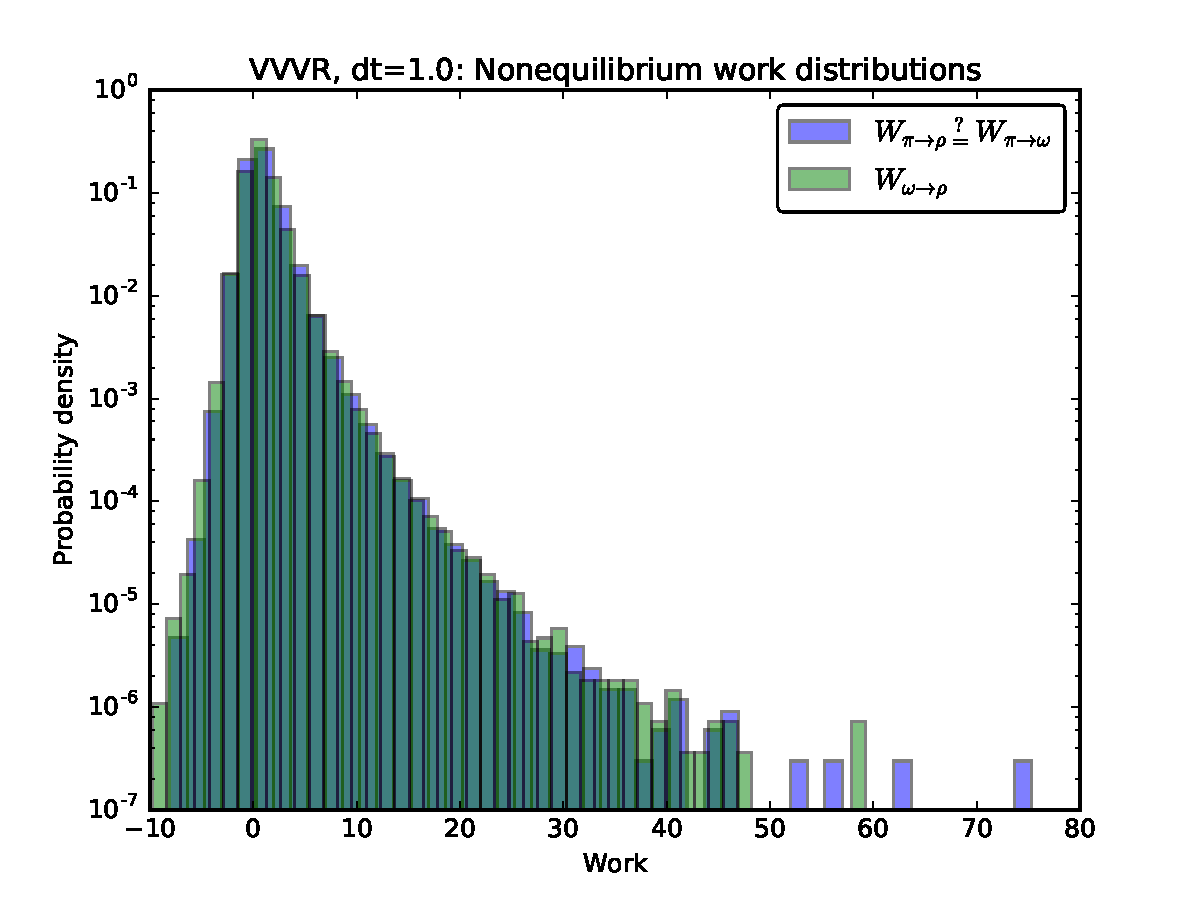
\includegraphics[width=\textwidth]{work_dists_VVVR_dt=1-0.pdf}
        \caption{$\delta t = 1$}
    \end{subfigure}
    \begin{subfigure}[b]{0.3\textwidth}
        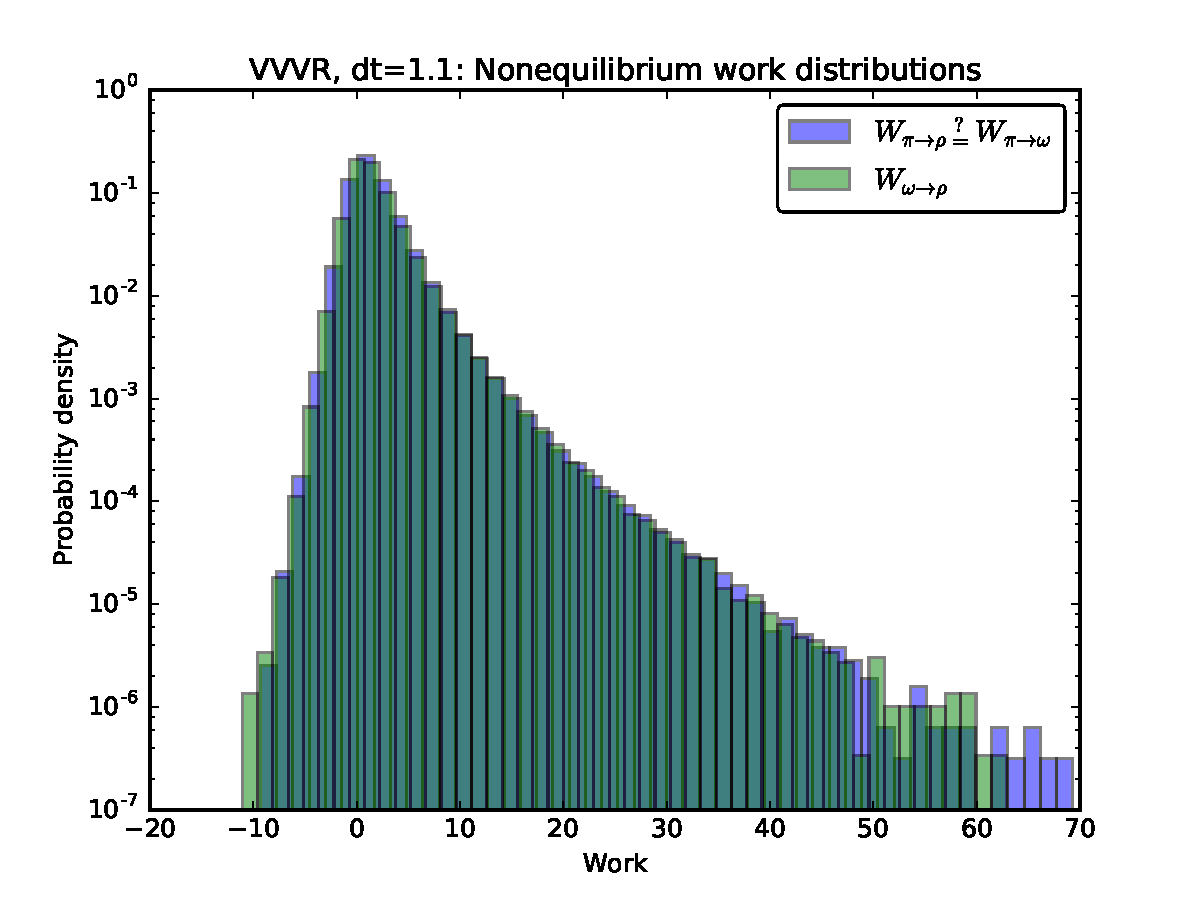
\includegraphics[width=\textwidth]{work_dists_VVVR_dt=1-1.pdf}
        \caption{$\delta t = 1.1$}
    \end{subfigure}
    \caption{VVVR work distributions}
\end{figure}

For this system, it looks like the differences between the ``forward'' and ``reverse'' work distributions are very slight, and these distributions also appear to have fatter tails with increasing step size.


\section{Molecular Mechanics Example}
To demonstrate that this approach is reasonable for molecular mechanics systems, we will use this procedure to estimate and compare the configuration-space bias of several Langevin integrators on a box of a few hundred TIP3P waters.

\end{document}
